\documentclass[12pt,letterpaper]{article}

% === TYPOGRAPHY ===
\usepackage[T1]{fontenc}
\usepackage[utf8]{inputenc}
\usepackage{mathptmx}  % Times New Roman for text and math
\usepackage{microtype}  % Better typography

% === PAGE LAYOUT ===
\usepackage{geometry}
\geometry{
    letterpaper,
    top=1in,
    bottom=1in,
    left=1.25in,
    right=1.25in,
    headheight=14pt
}

% === SPACING ===
\usepackage{setspace}
\doublespacing
\usepackage{parskip}
\setlength{\parskip}{0.5\baselineskip}
\setlength{\parindent}{0.5in}

% === HEADERS AND FOOTERS ===
\usepackage{fancyhdr}
\pagestyle{fancy}
\fancyhf{}
\fancyhead[R]{\small\thepage}
\renewcommand{\headrulewidth}{0pt}
\renewcommand{\footrulewidth}{0pt}

% === SECTION FORMATTING ===
\usepackage{titlesec}
\titleformat{\section}
    {\normalfont\Large\bfseries}
    {\thesection}{1em}{}
\titleformat{\subsection}
    {\normalfont\large\bfseries}
    {\thesubsection}{1em}{}
\titleformat{\subsubsection}
    {\normalfont\normalsize\bfseries}
    {\thesubsubsection}{1em}{}
\titleformat{\paragraph}[runin]
    {\normalfont\normalsize\bfseries}
    {}{0em}{}
\titlespacing*{\section}{0pt}{2\baselineskip}{1\baselineskip}
\titlespacing*{\subsection}{0pt}{1.5\baselineskip}{0.75\baselineskip}
\titlespacing*{\subsubsection}{0pt}{1\baselineskip}{0.5\baselineskip}
\titlespacing*{\paragraph}{0pt}{0.5\baselineskip}{1em}

% === TABLE OF CONTENTS ===
\usepackage{tocloft}
\renewcommand{\cftsecleader}{\cftdotfill{\cftdotsep}}
\setlength{\cftbeforesecskip}{0.5\baselineskip}
\setlength{\cftbeforesubsecskip}{0.25\baselineskip}

% === FIGURES AND CAPTIONS ===
\usepackage{graphicx}
\usepackage[font=small,labelfont=bf,labelsep=period]{caption}
\usepackage{float}

% === MATH ===
\usepackage{amsmath}
\usepackage{amssymb}

% === CITATIONS ===
\usepackage[numbers,sort&compress]{natbib}
\setlength{\bibsep}{0.5\baselineskip}

% === HYPERLINKS ===
\usepackage[hidelinks]{hyperref}
\usepackage{url}

% === ABSTRACT FORMATTING ===
\usepackage{abstract}
\renewcommand{\abstractnamefont}{\normalfont\Large\bfseries}
\setlength{\absleftindent}{0pt}
\setlength{\absrightindent}{0pt}

% === TITLE PAGE ===
\title{\vspace{-1in}\textbf{Consciousness as Constrained Biological Organization:\\[0.5\baselineskip]Entropy, Integration, and Formal Limits}}
\author{Christopher Ezernack}
\date{January 2026}

\begin{document}

\maketitle
\thispagestyle{empty}



\section*{Definitions}
\addcontentsline{toc}{section}{Definitions}

This paper employs several key concepts which require precise definition.\footnote{All conceptual figures created by the author are explanatory and non-empirical. Empirical results discussed in the text are drawn from cited peer-reviewed studies; figures from those studies are referenced via placeholders and may be inserted in future versions where licensing permits.}

\textbf{Formal System:} A system composed of a finite set of symbols and a set of rules for manipulating those symbols. In our context, a biological system is treated as a formal system wherein the symbols represent discrete biological states and the rules represent the physical and chemical laws governing transitions between those states.

\textbf{Entropy:} As used here, refers to degrees of freedom within a constrained subspace. High entropy corresponds to many simultaneously active configurations, while low entropy corresponds to constrained, stable configurations.

\textbf{Integration:} The irreducible unification of information across a system, such that the whole cannot be decomposed into independent parts without loss.

\textbf{Constraint:} Any process or condition that limits the degrees of freedom available to a system, thereby enforcing particular organizational regimes.

\textbf{Pruning:} The elimination of degrees of freedom, synaptic connections, or competing configurations, resulting in a more constrained and coherent system state.

\textbf{Gut-Brain Axis:} The bidirectional communication network connecting the central nervous system and the enteric nervous system, involving neural, endocrine, and immune pathways, and heavily influenced by the gut microbiome \cite{cryan2012}.

\textbf{Computational Irreducibility:} A property of some systems where the behavior cannot be predicted by any shortcut faster than simulating the system's evolution step by step \cite{wolfram2002}.

\begin{abstract}
\textbf{Problem Statement:} Neural activity alone is insufficient to explain stable, unified consciousness\footnote{Consciousness: Unified, subjective awareness characterized by phenomenal experience (qualia\footnote{Qualia: The subjective, qualitative properties of experience; the phenomenal character of what it is like to see red, feel pain, or hear a sound.}) and integrated self-reflection.}; substantial neural dynamics persist during sleep and anesthesia even as awareness collapses. This indicates that consciousness depends on organizational properties beyond local neural firing. A central problem is identifying the biological mechanisms that constrain neural degrees of freedom, enforce system-wide integration, and regulate entropy\footnote{Entropy: In this context, refers to the number of accessible microstates or degrees of freedom within a constrained system. High entropy corresponds to high variability and low organization; low entropy corresponds to low variability and high organization.} to stabilize a unified conscious state.

\textbf{Thesis:} This paper advances a conservative biological framework in which consciousness is treated as a stabilized organizational regime. We argue that neural systems require external biological constraints to achieve stable integration. The microbiota-gut-brain system is examined as a candidate constraint layer that shapes energetic and immune boundary conditions for neural viability, not as a generator of conscious content.

\textbf{Evidence Domains and Scope:} The framework is grounded in three evidence domains: (1) empirical findings from sleep, anesthesia, and perturbational complexity studies that measure integration and its loss; (2) formal arguments from logic and computation (Gödel, Penrose) suggesting the necessity of external constraint for system closure, applied here in a restricted, non-metaphysical sense; and (3) a review of the biophysical literature on microbial electromagnetic and oscillatory activity. We explicitly state that no direct evidence currently supports a specific gut-derived modulator frequency for neural pruning\footnote{Neural Pruning: The developmental and activity-dependent process by which synaptic connections are selectively eliminated to refine neural circuits, increase efficiency, and stabilize organization.}; this is framed as a targeted experimental opportunity, not a claim.

\textbf{Contribution:} The paper concludes with testable predictions and measurement strategies grounded in publicly established methods, aiming to bridge abstract theories of consciousness with concrete biological processes.
\end{abstract}

\newpage
\tableofcontents
\newpage

\section{Introduction and Problem Statement}

A central problem in consciousness research is explaining how biological systems achieve stable, unified awareness rather than fragmented or transient cognitive states. While decades of neuroscientific research have identified neural correlates associated with conscious experience, these correlates alone do not explain how integration is established or maintained. Neural activity can persist in the absence of awareness, as observed during deep sleep, general anesthesia, and certain pathological or dissociative states, indicating that consciousness depends on organizational properties beyond local neural firing \cite{koch2019, tononi2016}.

Increasing evidence suggests that consciousness is not tied to any single neural structure or signal, but to the global organization of activity across interacting subsystems. Network level modulation studies demonstrate that externally applied perturbations can reliably alter conscious state without modifying underlying anatomy. Transcranial magnetic stimulation and related perturbational approaches show that disrupting large scale integration can transiently collapse awareness even when neural activity remains present \cite{massimini2005, casali2013}. These findings indicate that consciousness is sensitive to constraint, coherence, and integration at the system level rather than to the mere presence of neural computation.

Taken together, these observations suggest that consciousness corresponds to a specific organizational regime rather than to a generative mechanism. Fragmented or hallucinatory cognitive states appear when many degrees of freedom\footnote{Degrees of Freedom: The number of independent parameters or variables required to specify the state of a system. In this context, refers to the number of possible neural configurations or activity patterns available to the brain.} remain active simultaneously, leading to unstable or competing patterns of organization. By contrast, unified conscious experience corresponds to a regime in which entropy is reduced, degrees of freedom are pruned, and global coherence is stabilized. Consciousness, in this sense, can be understood as a field like phenomenon arising from constrained integration rather than as a localized representation or process.

This leads to a central research question: what biological mechanisms are responsible for constraining neural degrees of freedom, enforcing system-wide integration, and regulating entropy to stabilize a unified conscious state? This paper advances the thesis that consciousness is a stabilized organizational regime that requires external biological constraint systems to achieve coherence. We argue that neural computation alone is insufficient to enforce its own organizational stability and that embodied regulatory networks, including the gut-brain axis, provide the necessary boundary conditions. The scope of this paper is to develop this framework, review the evidence for and against it, and outline testable predictions. The discussion of frequency-dependent phenomena is explicitly exploratory and evidence-seeking, not a claim of established mechanism.

One way to formalize this limitation is through the behavior of self referential systems. Systems that can be described in terms of internal states and transitions face inherent limits in their ability to fully determine their own closure conditions. Foundational results in logic demonstrate that sufficiently complex self referential systems cannot internally resolve all questions about their own operation, including which internal degrees of freedom should be eliminated to achieve stable closure \cite{godel1931, hofstadter1979}.\footnote{The invocation of Gödel’s incompleteness theorems does not imply that biological systems perform formal reasoning or symbolic mathematics. The relevance lies in the formal structure of systems that can be described in terms of discrete states and rule-governed transitions, which is sufficient for arithmetization and the applicability of incompleteness results, independent of determinism.} Applied biologically, this suggests that additional constraint systems may be required to regulate pruning and stabilization.

This motivates consideration of embodied regulatory processes that operate alongside but not within neural computation itself.\footnote{The argument here is not that neural computation is irrelevant, but that it is insufficient on its own to enforce the global coherence required for unified consciousness. External constraint systems provide the necessary boundary conditions for neural dynamics to settle into a stable, integrated state.} The gut brain biome represents a distributed biological network capable of influencing neural development, metabolism, immune signaling, and neurotransmitter availability \cite{cryan2012, foster2013}. These interactions occur across slower temporal scales and broader energetic domains than synaptic signaling, positioning the gut brain system as a plausible source of global constraint rather than localized computation.

An additional and underexplored dimension of such regulation concerns biological frequency organization. Neural dynamics are typically studied in low frequency bands accessible to electroencephalography, yet biological systems operate across a much wider range of temporal and energetic scales. Molecular vibrations, protein conformational dynamics, membrane oscillations, and collective modes in aqueous environments extend into the gigahertz and terahertz regimes \cite{froehlich1968, pokorny2004}. Bacterial systems in particular exhibit structured electromagnetic and vibrational activity associated with metabolism, ion transport, and collective organization. Whether such activity functions as an oscillator, a modulatory background, or a constraint field remains an open empirical question, but it offers a plausible domain in which non neural biological processes could influence neural coherence.

The problem addressed in this paper can therefore be stated clearly. Neural computation alone does not appear sufficient to explain the transition from primitive or fragmented cognition to unified conscious awareness. Network level modulation demonstrates that organization is critical, yet it does not identify the endogenous biological mechanisms responsible for enforcing that organization. We propose that external biological constraint systems, including gut brain ecological regulation and associated thermodynamic and frequency dependent processes, provide the conditions necessary for entropy reduction, pruning, and stable integration. This work develops a biologically grounded framework for understanding consciousness as an emergent field shaped by constraint and cross scale coupling, setting the stage for identifying concrete substrates and testable predictions.\footnote{The framework presented here is explicitly intended to be conservative and biologically grounded. It does not invoke new physics or speculative mechanisms, but rather seeks to explain consciousness through the interaction of known biological processes operating across different scales.}

\section{Entropy, Integration, and Biological Organization}

A useful way to approach consciousness without assuming a specific neural mechanism is to focus on entropy, integration, and constraint. Biological systems are inherently high dimensional, composed of many interacting elements operating across multiple spatial and temporal scales. Left unconstrained, such systems tend toward fragmentation, instability, or excessive variability. Conscious awareness, by contrast, is characterized phenomenologically by unity, continuity, and coherence. Any viable theory must therefore explain how large numbers of degrees of freedom are reduced and coordinated without eliminating functional differentiation.

Integrated Information Theory addresses this problem by proposing that consciousness corresponds to the extent to which a system is both differentiated and integrated, formalized by the quantity $\Phi$ \cite{tononi2004, tononi2016}. While $\Phi$ is often treated as a numerical measure, it can also be understood more generally as describing a regime in which information is irreducibly unified across the system. In this view, consciousness does not arise from the accumulation of information, but from the organization of information under constraint.

Here, we extend this interpretation by treating integrated information as an emergent property of entropy gradients shaped by biological regulation. Rather than locating consciousness in specific neurons or signals, integrated information is understood as a global organizational state in which entropy is sufficiently constrained to permit stable integration. High entropy states correspond to many simultaneously active configurations that compete without convergence, while low entropy states correspond to overly rigid or inactive systems. Conscious awareness emerges in an intermediate regime where entropy is reduced enough to allow coherence, but not so reduced that differentiation is lost.

This framing helps clarify why consciousness is sensitive to global organization rather than local activity. A system may exhibit substantial neural firing yet fail to generate awareness if entropy remains high and integration weak, as seen during dreaming sleep, anesthesia, or certain seizure states \cite{koch2019}. Conversely, modest neural activity organized under strong constraints can support coherent experience. The relevant variable is therefore not activity level, but the structure of interactions and the degree to which information is jointly constrained across the system.

Importantly, entropy regulation in biological systems is not purely neural. Energy availability, metabolic cost, thermodynamic limits, and slow regulatory processes all shape which neural configurations are viable. From this perspective, integrated information is not generated by neurons alone, but by the interaction between neural dynamics and embodied constraint systems that limit and guide those dynamics. Consciousness corresponds to the stabilization of this organizational state when entropy gradients are appropriately bounded.

This view also helps explain why consciousness is graded and state dependent. During deep sleep and under general anesthesia, large scale integration breaks down, entropy increases, and the coherent organizational state collapses or fragments \cite{massimini2005, casali2013}. Upon waking, slow regulatory processes restore constraints, allowing integration to reemerge. These transitions suggest that consciousness is not switched on by a specific signal, but arises when the system enters an admissible organizational regime.

Finally, treating consciousness as shaped by entropy gradients avoids strong metaphysical commitments. This approach does not imply a new fundamental force or substance. It describes a system level property that emerges when biological processes enforce sufficient constraint on information flow. In this sense, consciousness reflects a compressed, stabilized representation of underlying dynamics. The field metaphor is used here to capture coherence, continuity, and global coupling, not to assert an independent ontological entity.

\paragraph{Formal Limits of $\Phi$ and the Necessity of Biological Constraint}

Integrated Information Theory provides an important formal criterion for consciousness by restricting conscious systems to those that exhibit irreducible integration. Importantly, $\Phi$ is not an unconstrained or panpsychic quantity. As developed by Tononi and colleagues, it imposes strict bounds on what qualifies as conscious, excluding systems that lack causal integration, stable structure, or measurable interdependence among components \cite{tononi2016, oizumi2014}.

However, $\Phi$ does not specify how biological systems come to satisfy these constraints. The presence of integration is treated as a property to be measured, not a process to be explained. As a result, $\Phi$ alone does not account for the developmental, metabolic, or ecological mechanisms that stabilize integration over time.

In this framework, integrated information is interpreted as a measurable outcome of successful biological organization rather than as a generative principle. Entropy gradients, pruning processes, and constraint systems determine whether a system can enter and remain within a $\Phi$-admissible regime. Systems that lack such stabilizing mechanisms may transiently exhibit complex dynamics without achieving sustained integration. This interpretation explicitly excludes panpsychic extensions and conscious agents theories that treat $\Phi$ as an intrinsic property of all information processing systems.

\begin{figure}[htbp]
\centering
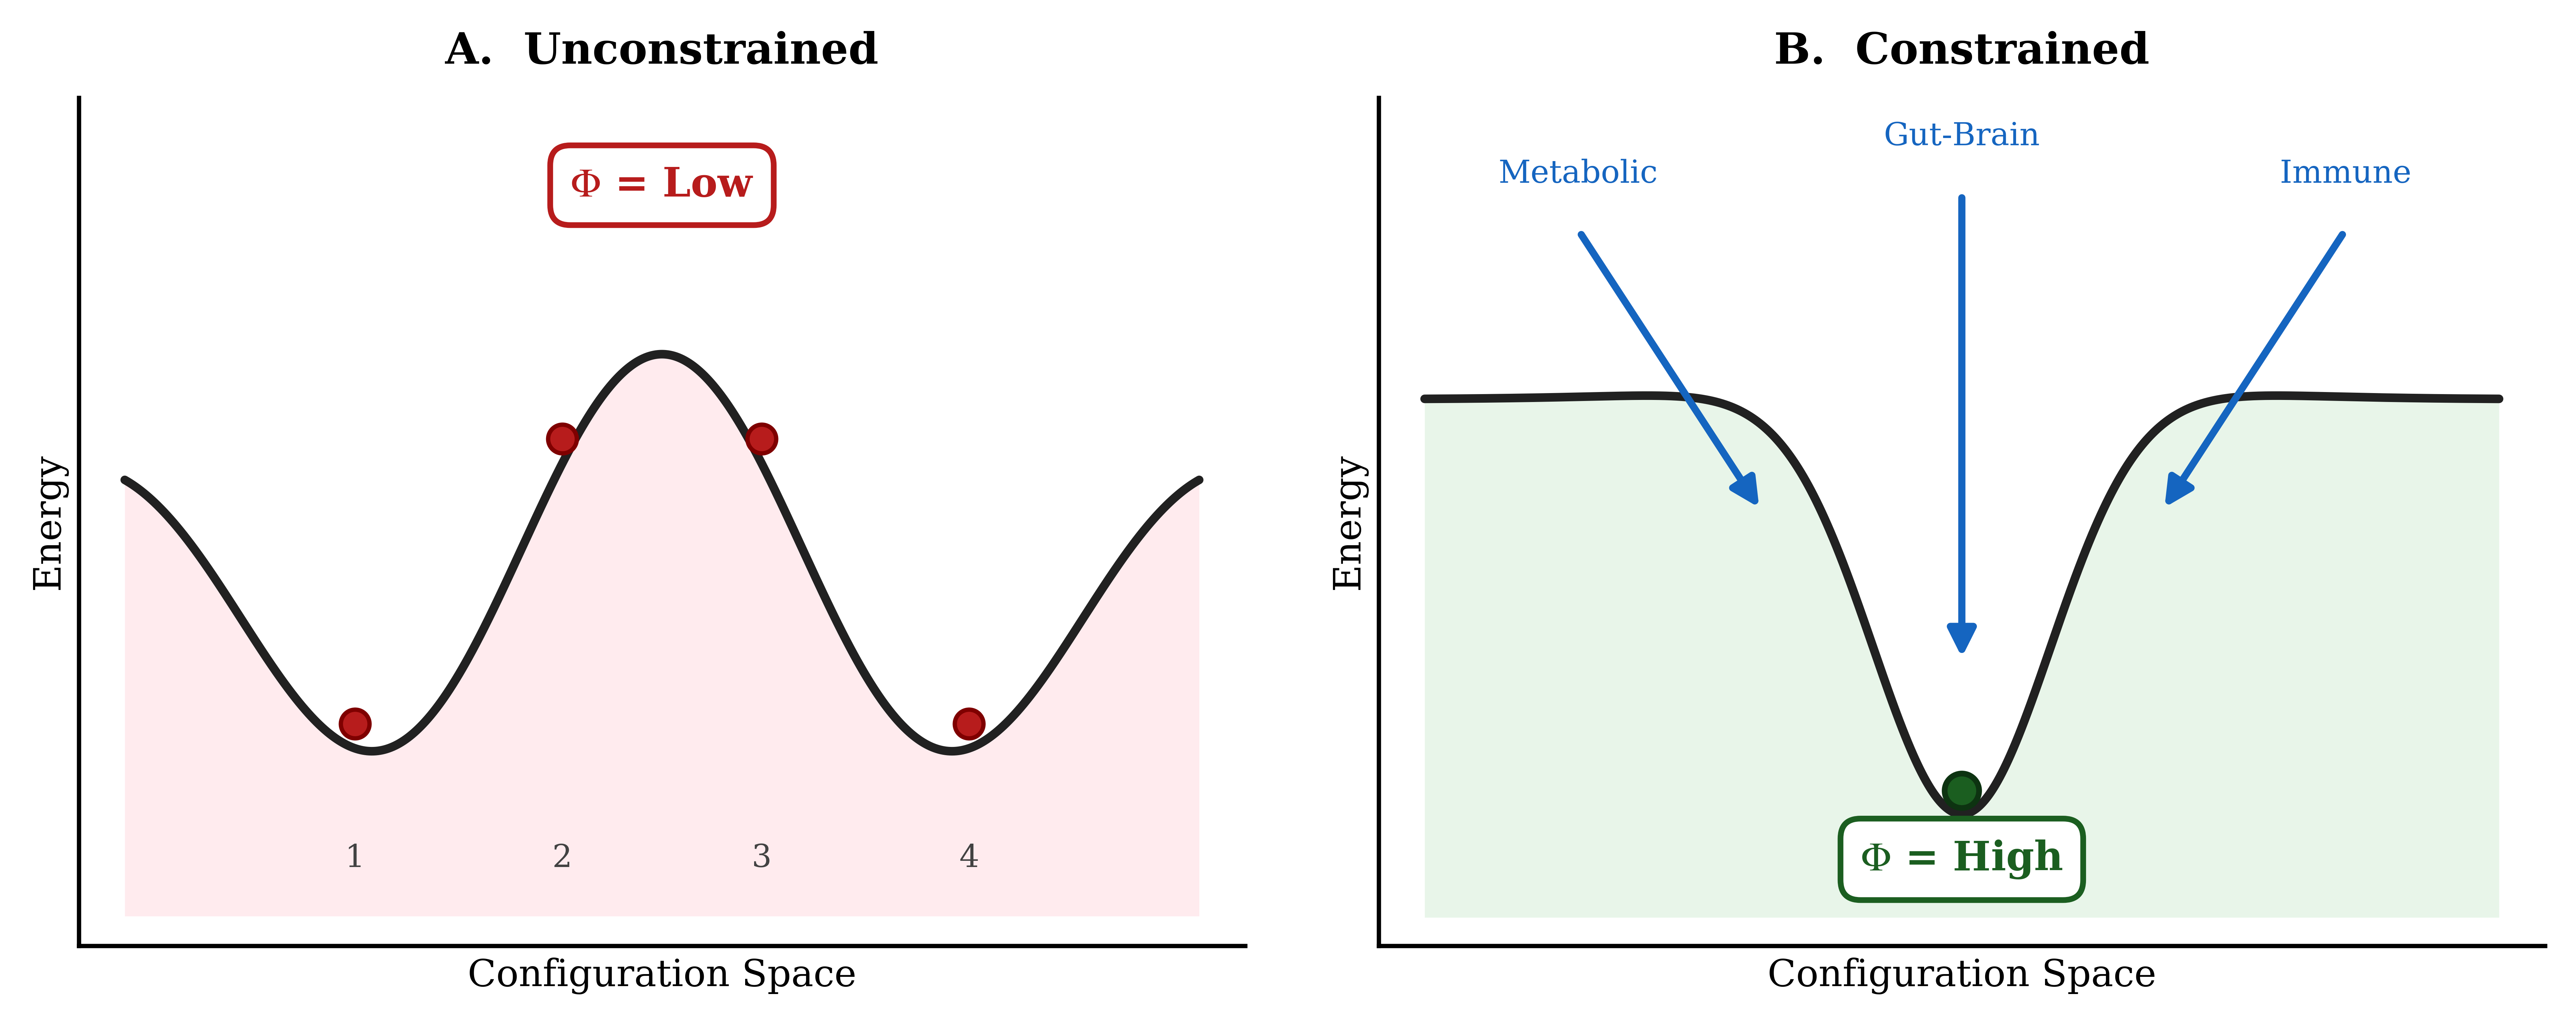
\includegraphics[width=\textwidth]{figure5_attractor_landscape.png}
\caption{Attractor stabilization and constraint-driven emergence of integrated conscious organization. A: Without external constraint, multiple internal attractors compete, resulting in fragmented dynamics and low integrated information ($\Phi$). B: External biological constraints (metabolic, immune, gut-brain regulation) deform the landscape, deepening a dominant basin and suppressing unstable attractors. $\Phi$ emerges as a measurable property of the stabilized configuration, not as a causal driver. \textit{Author-created conceptual diagram; non-empirical.}}
\label{fig:attractor_landscape}
\end{figure}

\begin{figure}[htbp]
\centering
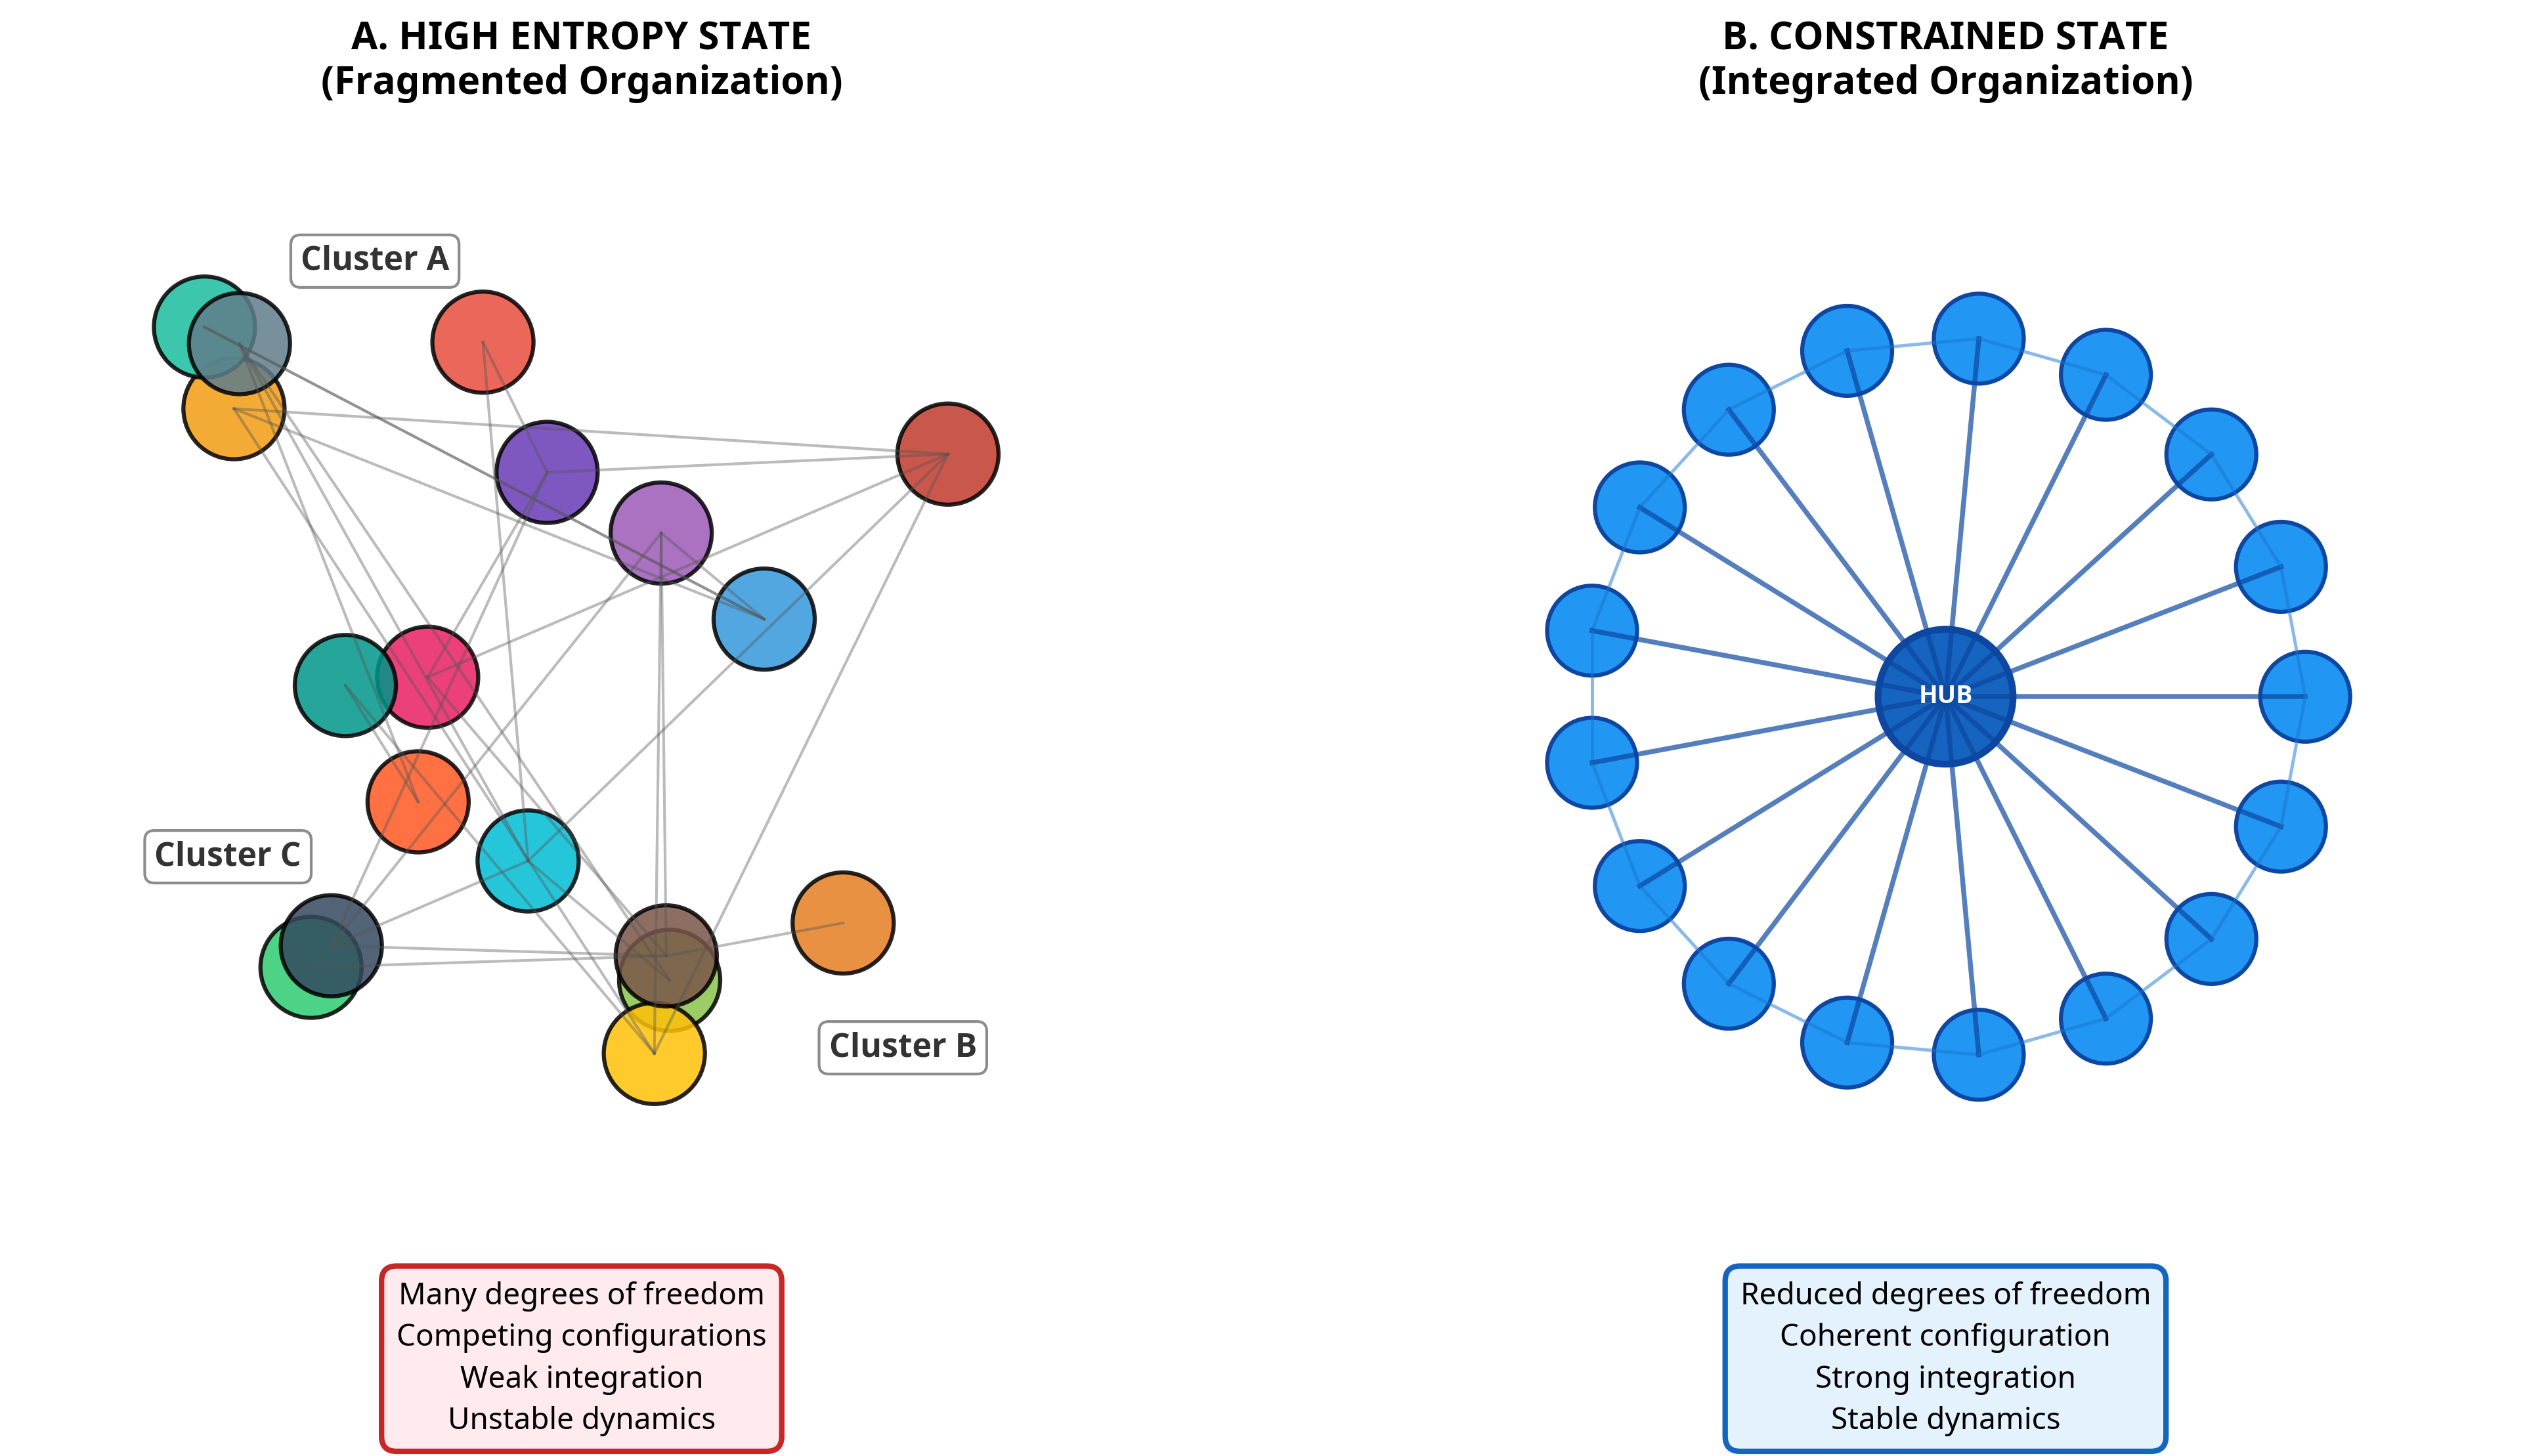
\includegraphics[width=\textwidth]{figure1_entropy_organization.png}
\caption{Conceptual schematic contrasting high entropy, fragmented neural organization (A) with constrained, integrated organization (B). In the high entropy state, multiple clusters operate with weak coupling and competing configurations, resulting in many degrees of freedom and unstable dynamics. In the constrained state, external biological regulation has reduced degrees of freedom, enabling coherent integration across the network with strong hub connectivity and stable dynamics. \textit{Author-created conceptual diagram; non-empirical; inspired by cited sources.}}
\label{fig:entropy_organization}
\end{figure}

\section{External Biological Constraint Systems}

If consciousness depends on entropy regulation, pruning, and large scale integration, then a central question concerns the biological origin of these constraints. Neural networks are highly adaptive and capable of generating complex internal dynamics, but plasticity alone does not guarantee convergence. Without mechanisms that limit degrees of freedom and enforce energetic and organizational viability, neural activity may remain fragmented or unstable. This suggests that additional biological systems are required to supply constraints that neural computation alone cannot fully impose.

One such system is the gut brain biome. The gastrointestinal tract hosts a dense and metabolically active microbial ecosystem that interacts continuously with the nervous system through immune signaling, metabolic pathways, vagal afferents, and neuroactive compounds \cite{cryan2012, foster2013}. These interactions influence neural development, synaptic plasticity, stress reactivity, and cognitive function across the lifespan. Importantly, the gut brain system operates on slower temporal scales and broader energetic domains than synaptic signaling, positioning it as a regulator rather than a computational substrate.\footnote{The microbiota–gut–brain axis is discussed as a modulatory biological system influencing immune, metabolic, and neural boundary conditions. No claim is made that microbial activity constitutes conscious processing or generates conscious content.}

From the perspective developed here, the gut brain biome does not generate conscious content. Instead, it contributes to shaping the space of viable neural configurations by imposing energetic, metabolic, and thermodynamic constraints. Microbial metabolism affects the availability of neurotransmitter precursors, modulates inflammatory states, and influences mitochondrial efficiency. These factors alter the energetic cost of neural activity and thereby bias which patterns of activity can be sustained over time. In this way, the gut brain system can indirectly enforce pruning by rendering certain neural configurations metabolically unfavorable.

Such embodied regulation is consistent with the idea that consciousness emerges only when degrees of freedom are sufficiently constrained. Primitive or unstable cognitive states may reflect regimes in which constraint is weak, allowing many competing internal models to coexist. As regulatory systems mature or stabilize, entropy gradients become steeper, pruning intensifies, and coherent integration becomes possible. This framing aligns with developmental evidence showing that both neural pruning and microbiome composition change dramatically during early life, coinciding with the emergence of stable cognitive organization \cite{johnson2018, kundu2017}.

External constraint systems are not limited to the gut brain axis. Thermodynamic factors such as temperature regulation, oxygen availability, and pressure also play a role in shaping neural viability. Biological systems must dissipate heat, maintain chemical gradients, and operate within narrow physical limits. Neural activity that exceeds these limits cannot persist. These constraints act globally and continuously, providing a background against which neural dynamics unfold. Rather than being incidental, such physical limits may be essential for enforcing the entropy bounds required for coherent awareness.

Another dimension of constraint concerns biological frequency organization. While neural oscillations are typically studied in low frequency bands, biological processes extend across a much wider spectrum. Molecular vibrations, protein conformational changes, membrane dynamics, and collective oscillatory modes in water occur at much higher frequencies, including the gigahertz and terahertz ranges \cite{froehlich1968, pokorny2004}. Bacterial systems in particular exhibit coordinated electromagnetic and vibrational behavior linked to metabolism, ion transport, and collective organization.

At present, it is not known whether such high frequency biological activity functions as a discrete oscillator, a modulatory background, or a constraint field influencing neural coherence. This paper does not claim the existence of a specific consciousness frequency. Instead, it highlights the possibility that non neural biological processes operating at higher frequencies contribute indirectly by stabilizing lower frequency neural integration. In this view, frequency organization is not a cause of consciousness, but a potential marker or enabling condition for constraint mediated coherence.

\paragraph{Internal and External Attractors in Conscious Organization}

Self-organizing biological systems naturally form internal attractor states corresponding to stable patterns of activity. However, internal attractors alone are insufficient to guarantee coherent integration. Without constraint, multiple attractors may compete, leading to fragmentation, hallucination, or unstable cognition.

External biological constraint systems provide directional pressure that biases attractor landscapes toward viable configurations. The gut-brain biome functions as one such external attractor, influencing metabolic cost, immune tone, and pruning dynamics. Rather than encoding content, these external influences shape which internal attractors remain energetically and developmentally accessible.

Conscious organization emerges when internal neural attractors are stabilized and pruned under sustained external constraint, enabling persistent self-referential processing and integration. In this view, $\Phi$ reflects the outcome of this alignment rather than its cause. The entropy gradients and self-organizing dynamics that characterize neural systems are shaped by external attractors such as gut bacteria, which modulate the conditions under which viable, integrated configurations can persist.

Taken together, these considerations suggest that consciousness arises within a broader biological context in which neural dynamics are shaped by multiple interacting constraint systems. The gut brain biome, thermodynamic regulation, and frequency dependent biological organization collectively limit degrees of freedom, enforce pruning, and stabilize integration. Conscious awareness emerges when these constraints align to support a coherent, low entropy organizational regime. Identifying and characterizing these substrates is therefore essential for moving from abstract theories of consciousness toward biologically grounded mechanisms.

\begin{figure}[htbp]
\centering
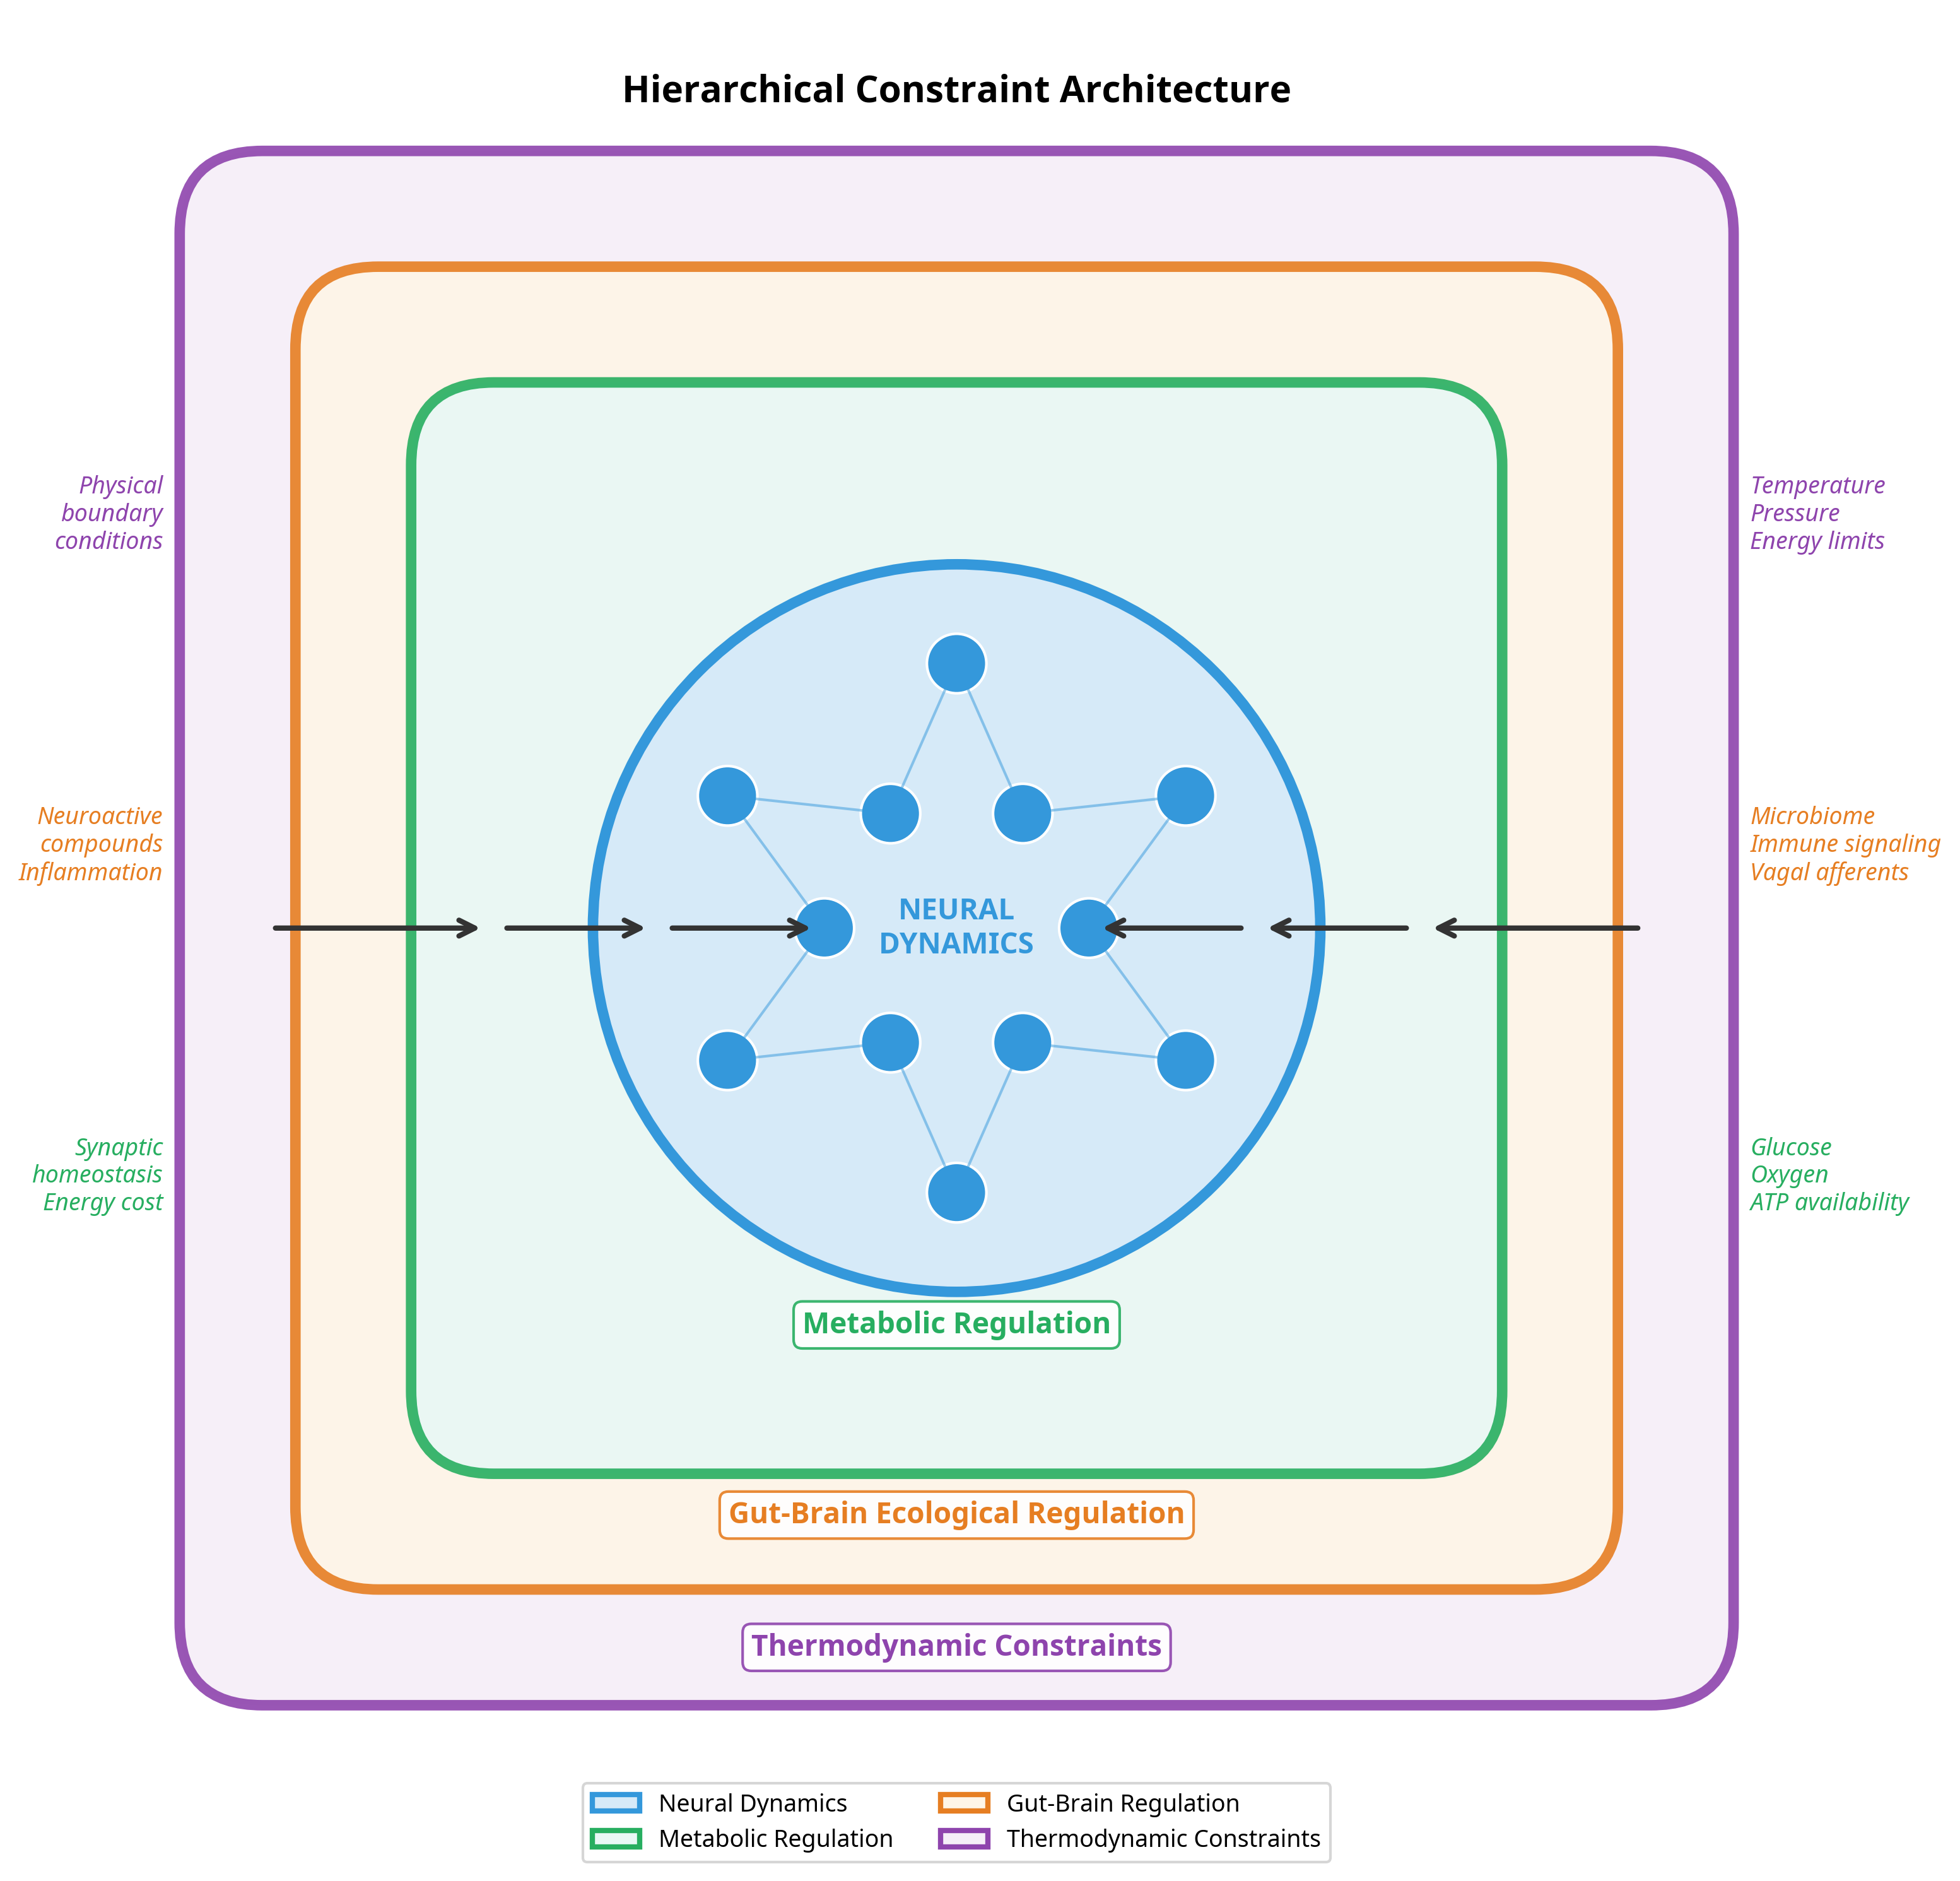
\includegraphics[width=0.85\textwidth]{figure2_constraint_layers.png}
\caption{Hierarchical constraint architecture showing the relationship between neural dynamics and external biological regulation. Neural dynamics (center) are embedded within successive layers of constraint: metabolic regulation (controlling glucose, oxygen, and ATP availability), gut-brain ecological regulation (including microbiome signaling, immune pathways, and vagal afferents), and thermodynamic constraints (temperature, pressure, and energy limits). Arrows indicate the direction of constraint, flowing inward from outer layers to shape the space of viable neural configurations. \textit{Author-created conceptual diagram; non-empirical; inspired by cited sources.}}
\label{fig:constraint_layers}
\end{figure}

\section{Formal Arithmetization, Discrete Outcomes, and the Applicability of G\"{o}del Limits}

A central claim of this work is that biological systems relevant to consciousness can be treated, at an appropriate level of description, as systems composed of discrete states and transitions. This claim does not assert classical determinism, nor does it deny probabilistic dynamics at the quantum or molecular level. Rather, it reflects the fact that biological function depends on realized outcomes rather than on superposed possibilities.

At the scale relevant to biological organization, physical processes resolve into definite events. Molecular interactions either occur or do not occur. Ion channels open or remain closed. Binding events succeed or fail. Even in quantum mechanics, measurements of quantities such as spin or energy yield discrete eigenvalues. While the underlying dynamics may be probabilistic, biological systems operate on the basis of actualized events rather than probability amplitudes. As a result, biological processes can be described in terms of discrete state changes governed by constraints.

The applicability of Gödel's incompleteness theorems to physical and biological systems is approached here with caution. The argument does not require treating the brain as a Turing machine. Instead, it rests on a series of conservative premises:

\begin{enumerate}
    \item Biological systems operate on realized events; their states can be described as a sequence of discrete outcomes (e.g., a neuron either fires or it does not; a gene is either expressed or it is not). 
    \item Any system of discrete outcomes permits a symbolic description, where symbols represent states and rules represent transitions.
    \item Any sufficiently expressive symbolic system can be arithmetized, mapping its statements onto numbers, making it subject to formal analysis.
    \item Gödel's theorems apply to any such formal system, demonstrating that it cannot internally prove its own consistency or decide all statements about itself. This applies regardless of whether the system's rules are deterministic or probabilistic. Quantum indeterminacy does not invalidate the formal limits of the descriptive system.
\end{enumerate}

This chain of reasoning leads to a key defensive clarification. The argument is about the limits of formal closure, not metaphysical determinism. We use Penrose's work here only to block the common but incorrect objection that quantum mechanics provides a loophole to incompleteness. The argument does not require the Orch OR model to be correct. It simply posits that if a biological system's behavior can be described formally, it cannot be its own sole guarantor of stability. It requires an external constraint to prune its state space and enforce a globally coherent regime.\footnote{Penrose is cited here solely to address the common objection that quantum indeterminacy exempts physical systems from formal limitations. This paper does not rely on Orch OR or any specific quantum collapse model, nor does it claim that consciousness itself causes state reduction.}

This leads to a key conclusion. If neural and biological subsystems cannot internally resolve all questions concerning their own organization, then stable convergence requires constraints imposed by processes operating outside the system's own representational layer. Pruning, entropy reduction, and stabilization must therefore be enforced by embodied biological constraint systems rather than by neural computation alone. Conscious organization emerges when such constraints succeed in collapsing degrees of freedom into a coherent, integrated regime.

\section{Sleep and Anesthesia as Natural Experiments in Constraint Loss and Restoration}

Sleep and anesthesia provide natural experimental conditions for examining how conscious organization depends on constraint, integration, and entropy regulation. Unlike focal brain lesions or artificial stimulation, these states alter global organization while largely preserving underlying neural structures. As such, they offer insight into which properties of biological systems are necessary for unified awareness.

During deep sleep, particularly slow wave sleep, the brain exhibits a characteristic breakdown in effective connectivity. Transcranial magnetic stimulation applied during this state produces short lived, localized cortical responses rather than the complex, distributed patterns observed during wakefulness \cite{massimini2005}. This indicates that the capacity for large scale integration is diminished, even though neurons remain active. The perturbational complexity index, a measure designed to quantify the information content of cortical responses, reliably distinguishes between conscious and unconscious states by capturing this loss of integrated complexity \cite{casali2013}.

General anesthesia produces a similar but more pronounced effect. Across a range of anesthetic agents, loss of consciousness is associated with a breakdown in information integration, loss of long range communication, and collapse of network complexity \cite{alkire2008, sanders2012}. Perturbational studies show that anesthetized brains respond to stimulation with short lived, localized activity rather than sustained, distributed patterns, indicating a failure to maintain coherent organization \cite{casali2013}.

These findings align with the view that consciousness corresponds to an admissible organizational regime rather than to a particular level of activity. Under sleep and anesthesia, entropy increases at the global level as degrees of freedom become decoupled, even though local order may persist. The system fails to converge on a single coherent configuration, and the integrated organizational structure associated with unified awareness collapses. This is empirically demonstrated by studies showing the breakdown of cortical effective connectivity during NREM sleep \cite{massimini2005} and the sharp decline in the Perturbational Complexity Index (PCI) during both sleep and anesthesia \cite{casali2013, casarotto2016}.

\begin{figure}[htbp]
\centering
\fbox{
  \parbox{0.8\textwidth}{
    \centering
    \vspace{2cm}
    Figure placeholder: TMS-evoked EEG responses showing breakdown of cortical effective connectivity across wake, NREM, and REM sleep.
    \vspace{1cm}
    \\
    \textit{Source: Massimini et al. (2005, 2010)}
    \vspace{2cm}
  }
}
\caption{Placeholder for empirical figure demonstrating the collapse of effective connectivity during NREM sleep as measured by TMS-EEG. The figure would show widespread, complex responses during wakefulness and REM sleep, contrasting with simple, local responses during NREM sleep.}
\label{fig:placeholder_massimini}
\end{figure}

\begin{figure}[htbp]
\centering
\fbox{
  \parbox{0.8\textwidth}{
    \centering
    \vspace{2cm}
    Figure placeholder: Perturbational Complexity Index (PCI) values across states of consciousness.
    \vspace{1cm}
    \\
    \textit{Source: Casali et al. (2013), Casarotto et al. (2016)}
    \vspace{2cm}
  }
}
\caption{Placeholder for empirical figure summarizing PCI values. The figure would show high PCI values for conscious states (wakefulness, REM sleep, locked-in syndrome) and low PCI values for unconscious states (NREM sleep, general anesthesia, vegetative state), establishing an empirical threshold for consciousness.}
\label{fig:placeholder_pci}
\end{figure}

Importantly, the transition into and out of these states is not driven solely by neural dynamics. Sleep onset and recovery involve slow, embodied regulatory processes including metabolic changes, neuromodulatory shifts, and circadian influences. Similarly, emergence from anesthesia depends on systemic factors such as drug clearance, thermoregulation, and restoration of metabolic balance. These observations suggest that global constraint systems play a central role in restoring the conditions required for integration.

Sleep also appears to serve an active regulatory function. Slow wave sleep is associated with synaptic downscaling, pruning, and redistribution of neural resources, processes thought to reduce entropy and prevent runaway excitation \cite{tononi2014}. From the perspective developed here, sleep can be understood as a controlled period of constraint relaxation followed by reimposition, allowing the system to reset and reestablish coherent organization. Conscious awareness reemerges not because neural activity resumes, but because constraints are restored to an admissible range.

Together, sleep and anesthesia demonstrate that conscious awareness is fragile with respect to global organization and constraint. They show that biological systems can enter states in which neural computation continues but consciousness is absent due to a failure of integration. These natural experiments support the broader claim that consciousness arises only when external and embodied regulatory processes enforce sufficient entropy reduction, pruning, and coherence across the system.

\begin{figure}[htbp]
\centering
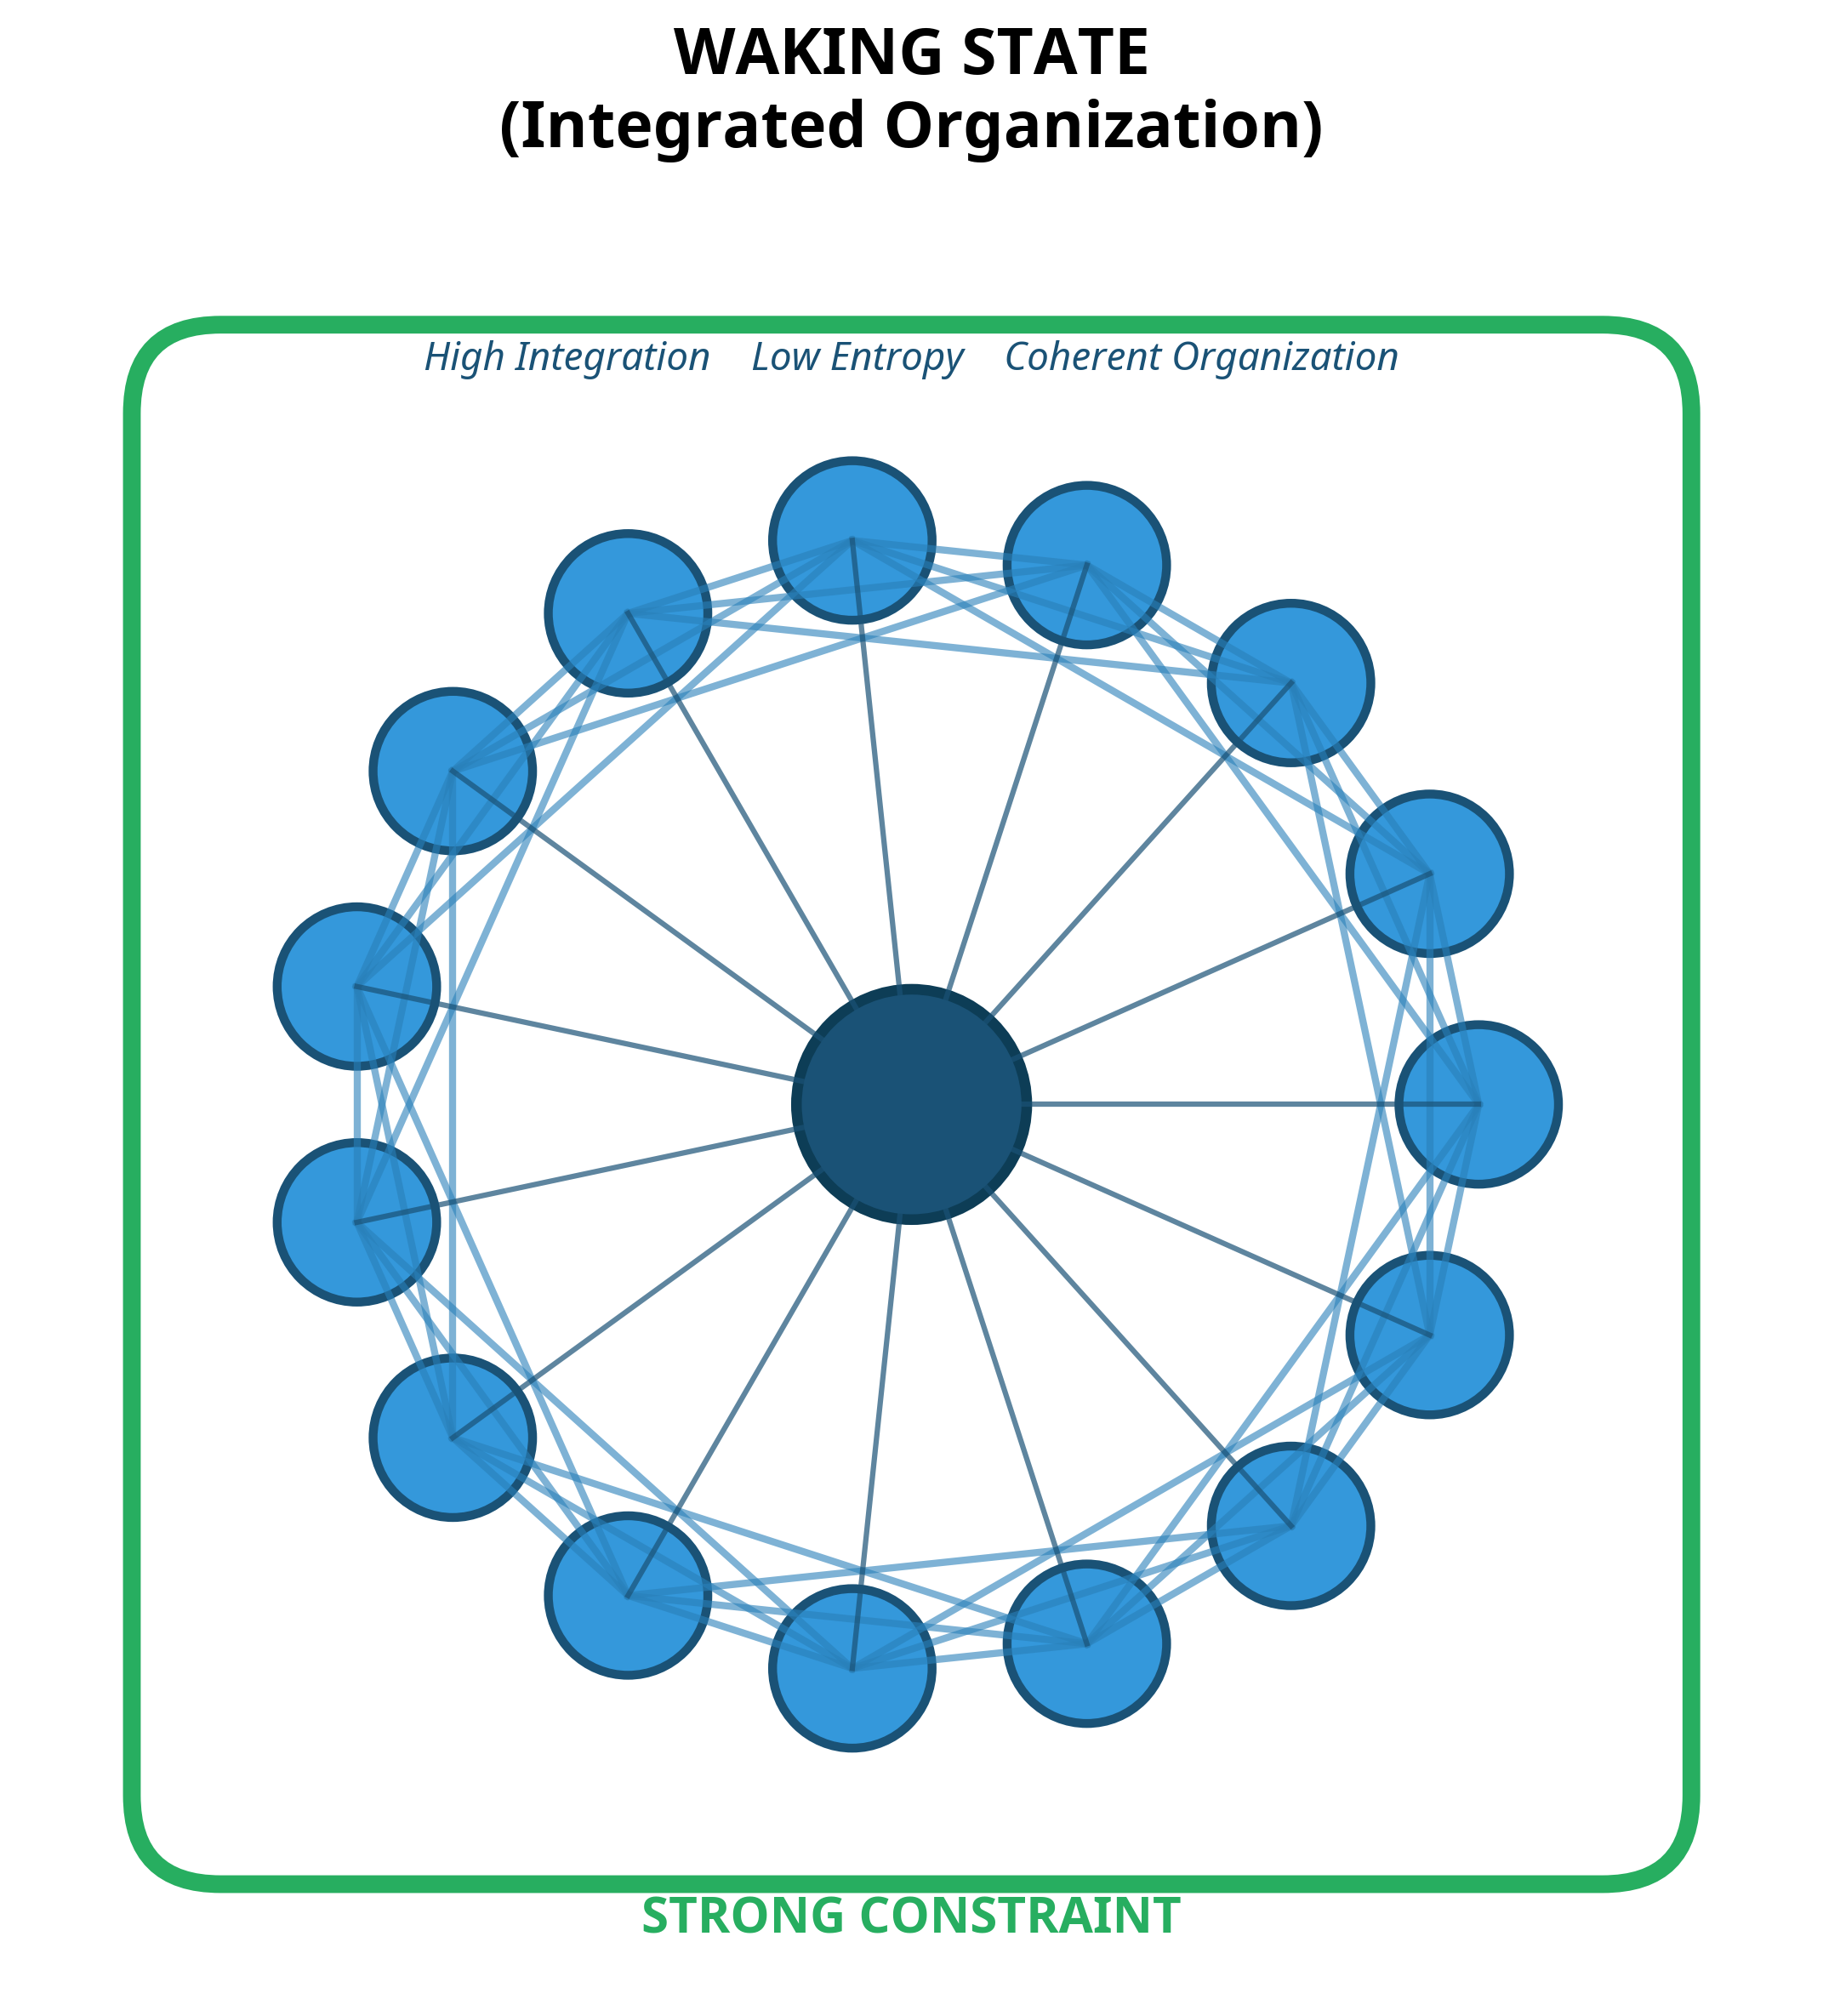
\includegraphics[width=0.7\textwidth]{figure3a_waking.png}
\caption{Waking state organization. During normal waking consciousness, neural dynamics exhibit high integration with strong hub connectivity. External biological constraints maintain low entropy and coherent organization across the network. The solid border represents strong constraint conditions that support unified awareness. \textit{Author-created conceptual diagram; non-empirical; inspired by cited sources.}}
\label{fig:waking}
\end{figure}

\begin{figure}[htbp]
\centering
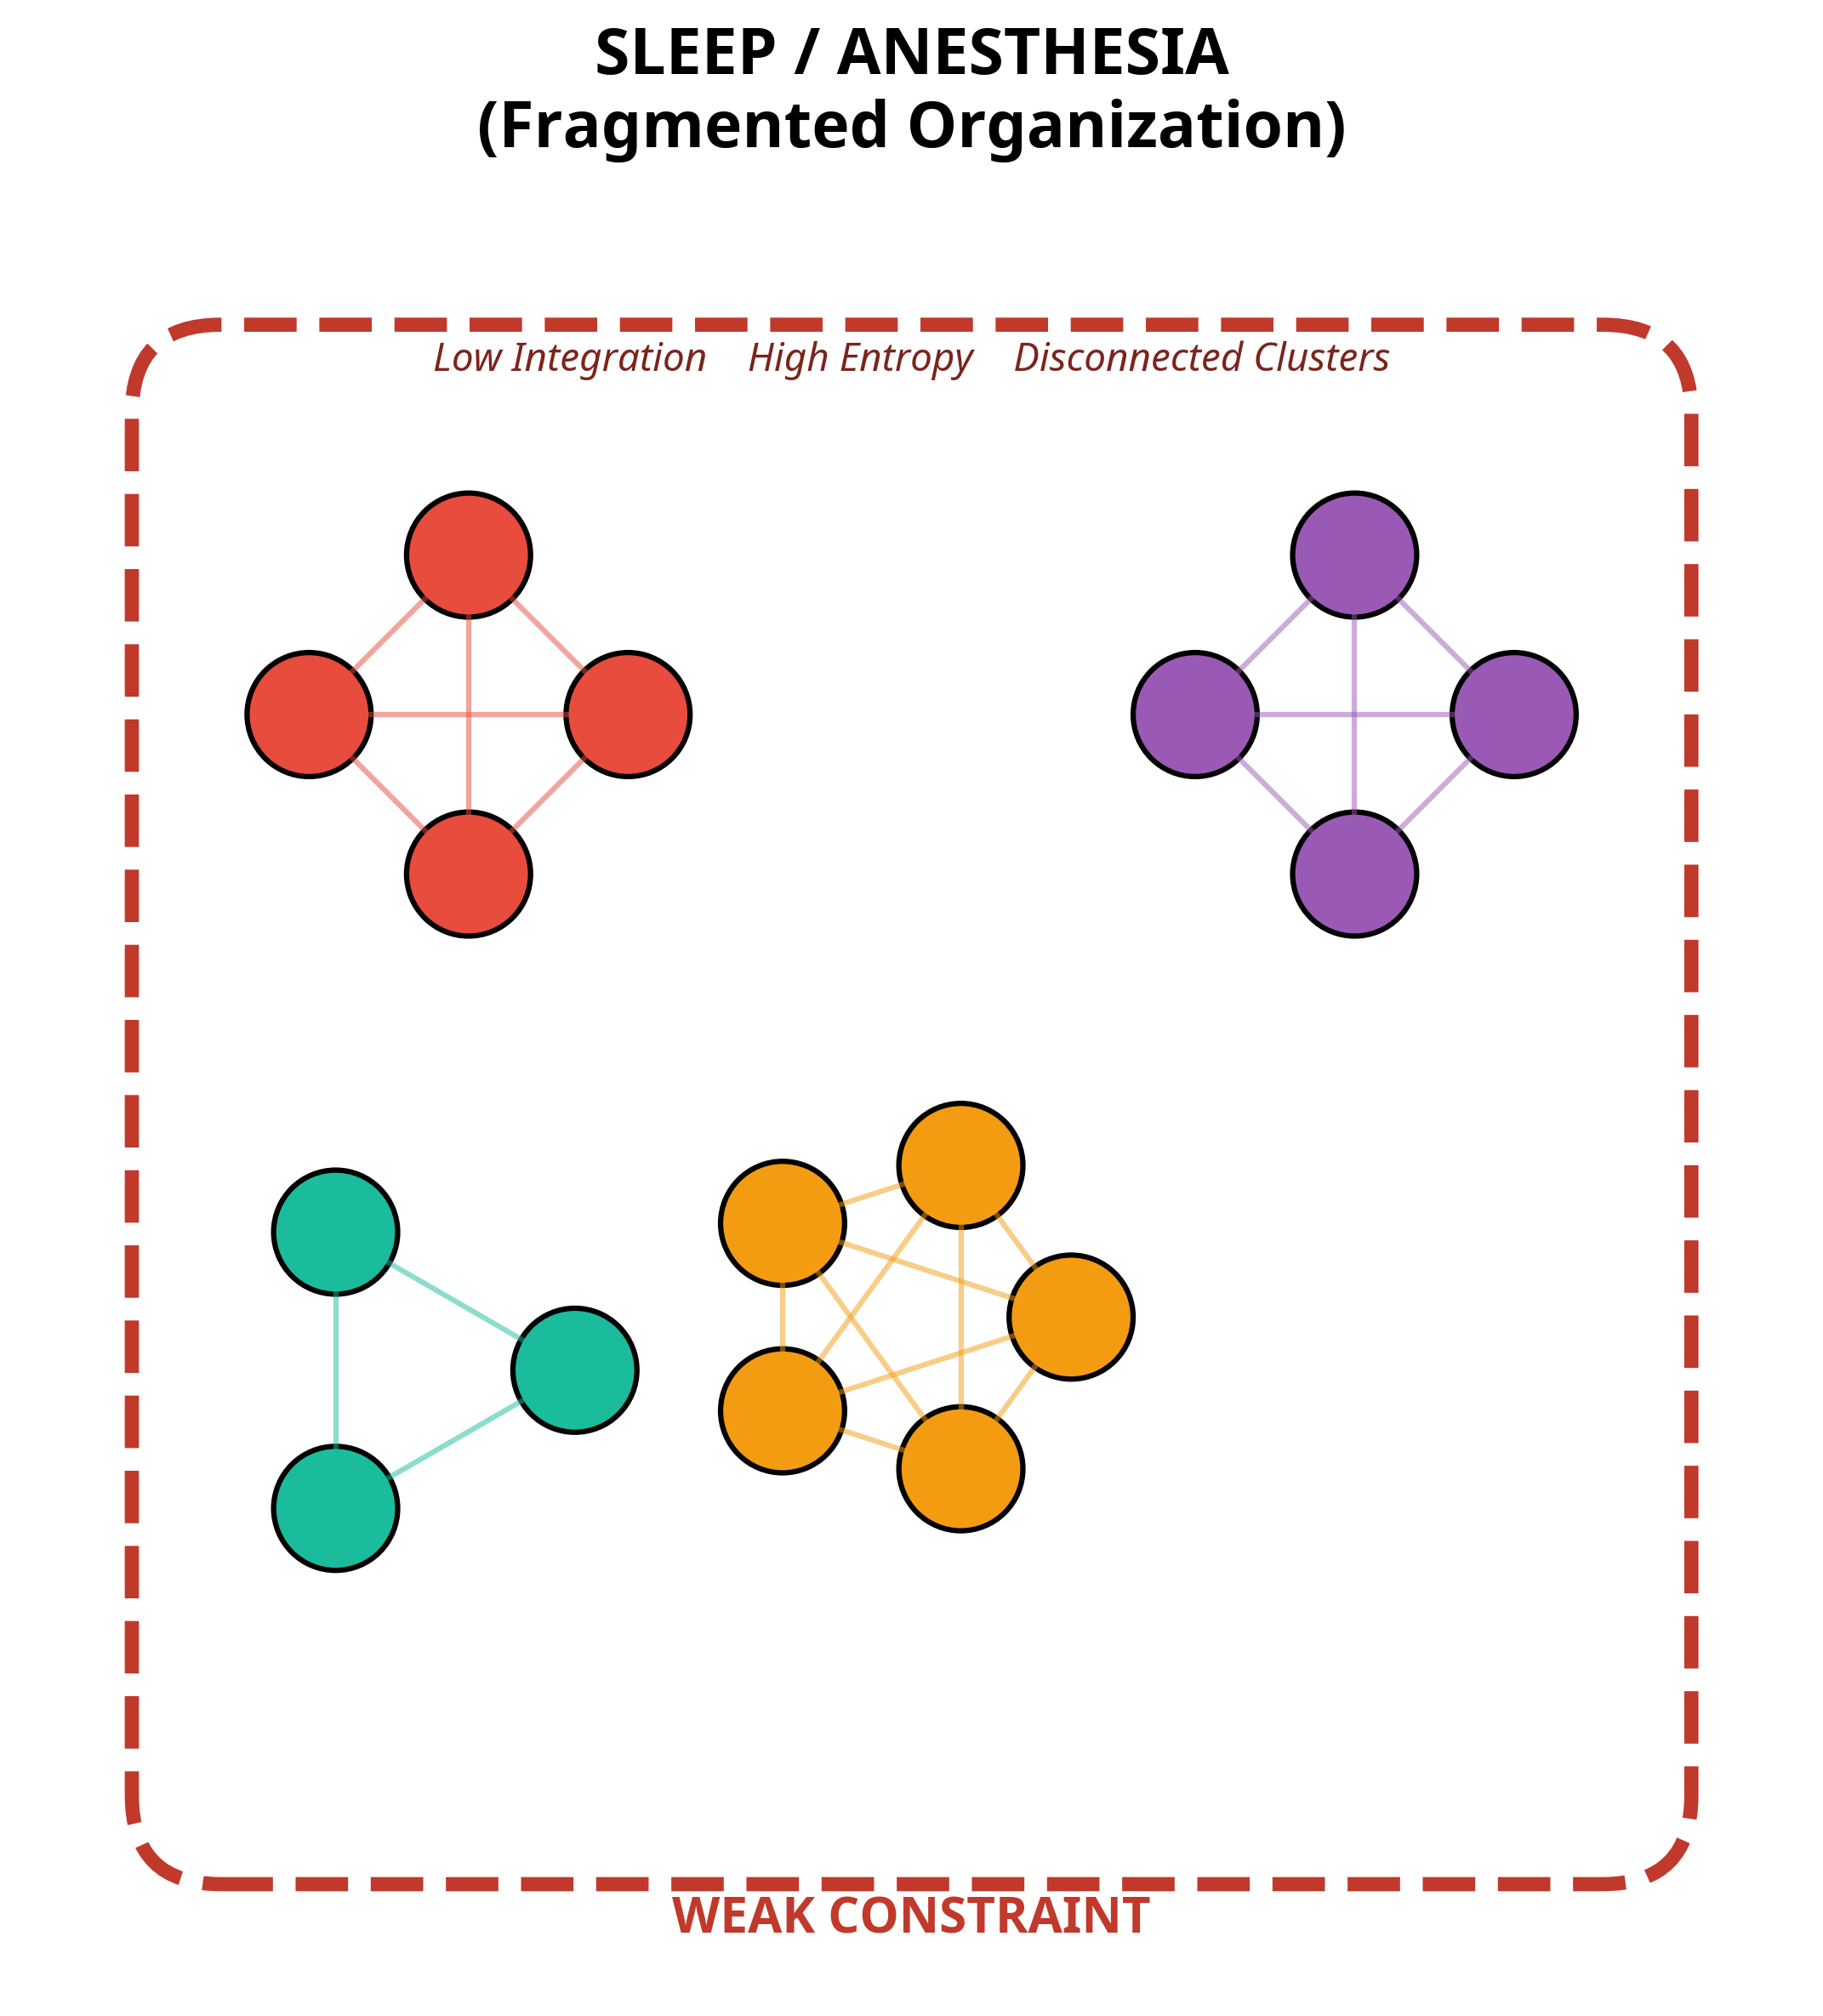
\includegraphics[width=0.7\textwidth]{figure3b_fragmented.png}
\caption{Sleep and anesthesia state organization. During deep sleep and general anesthesia, neural organization fragments into disconnected clusters. Integration collapses as constraint weakens, resulting in high entropy and loss of coherent awareness. The dashed border represents weak constraint conditions. Multiple independent subsystems operate without convergence on a unified configuration. \textit{Author-created conceptual diagram; non-empirical; inspired by cited sources.}}
\label{fig:fragmented}
\end{figure}

\begin{figure}[htbp]
\centering
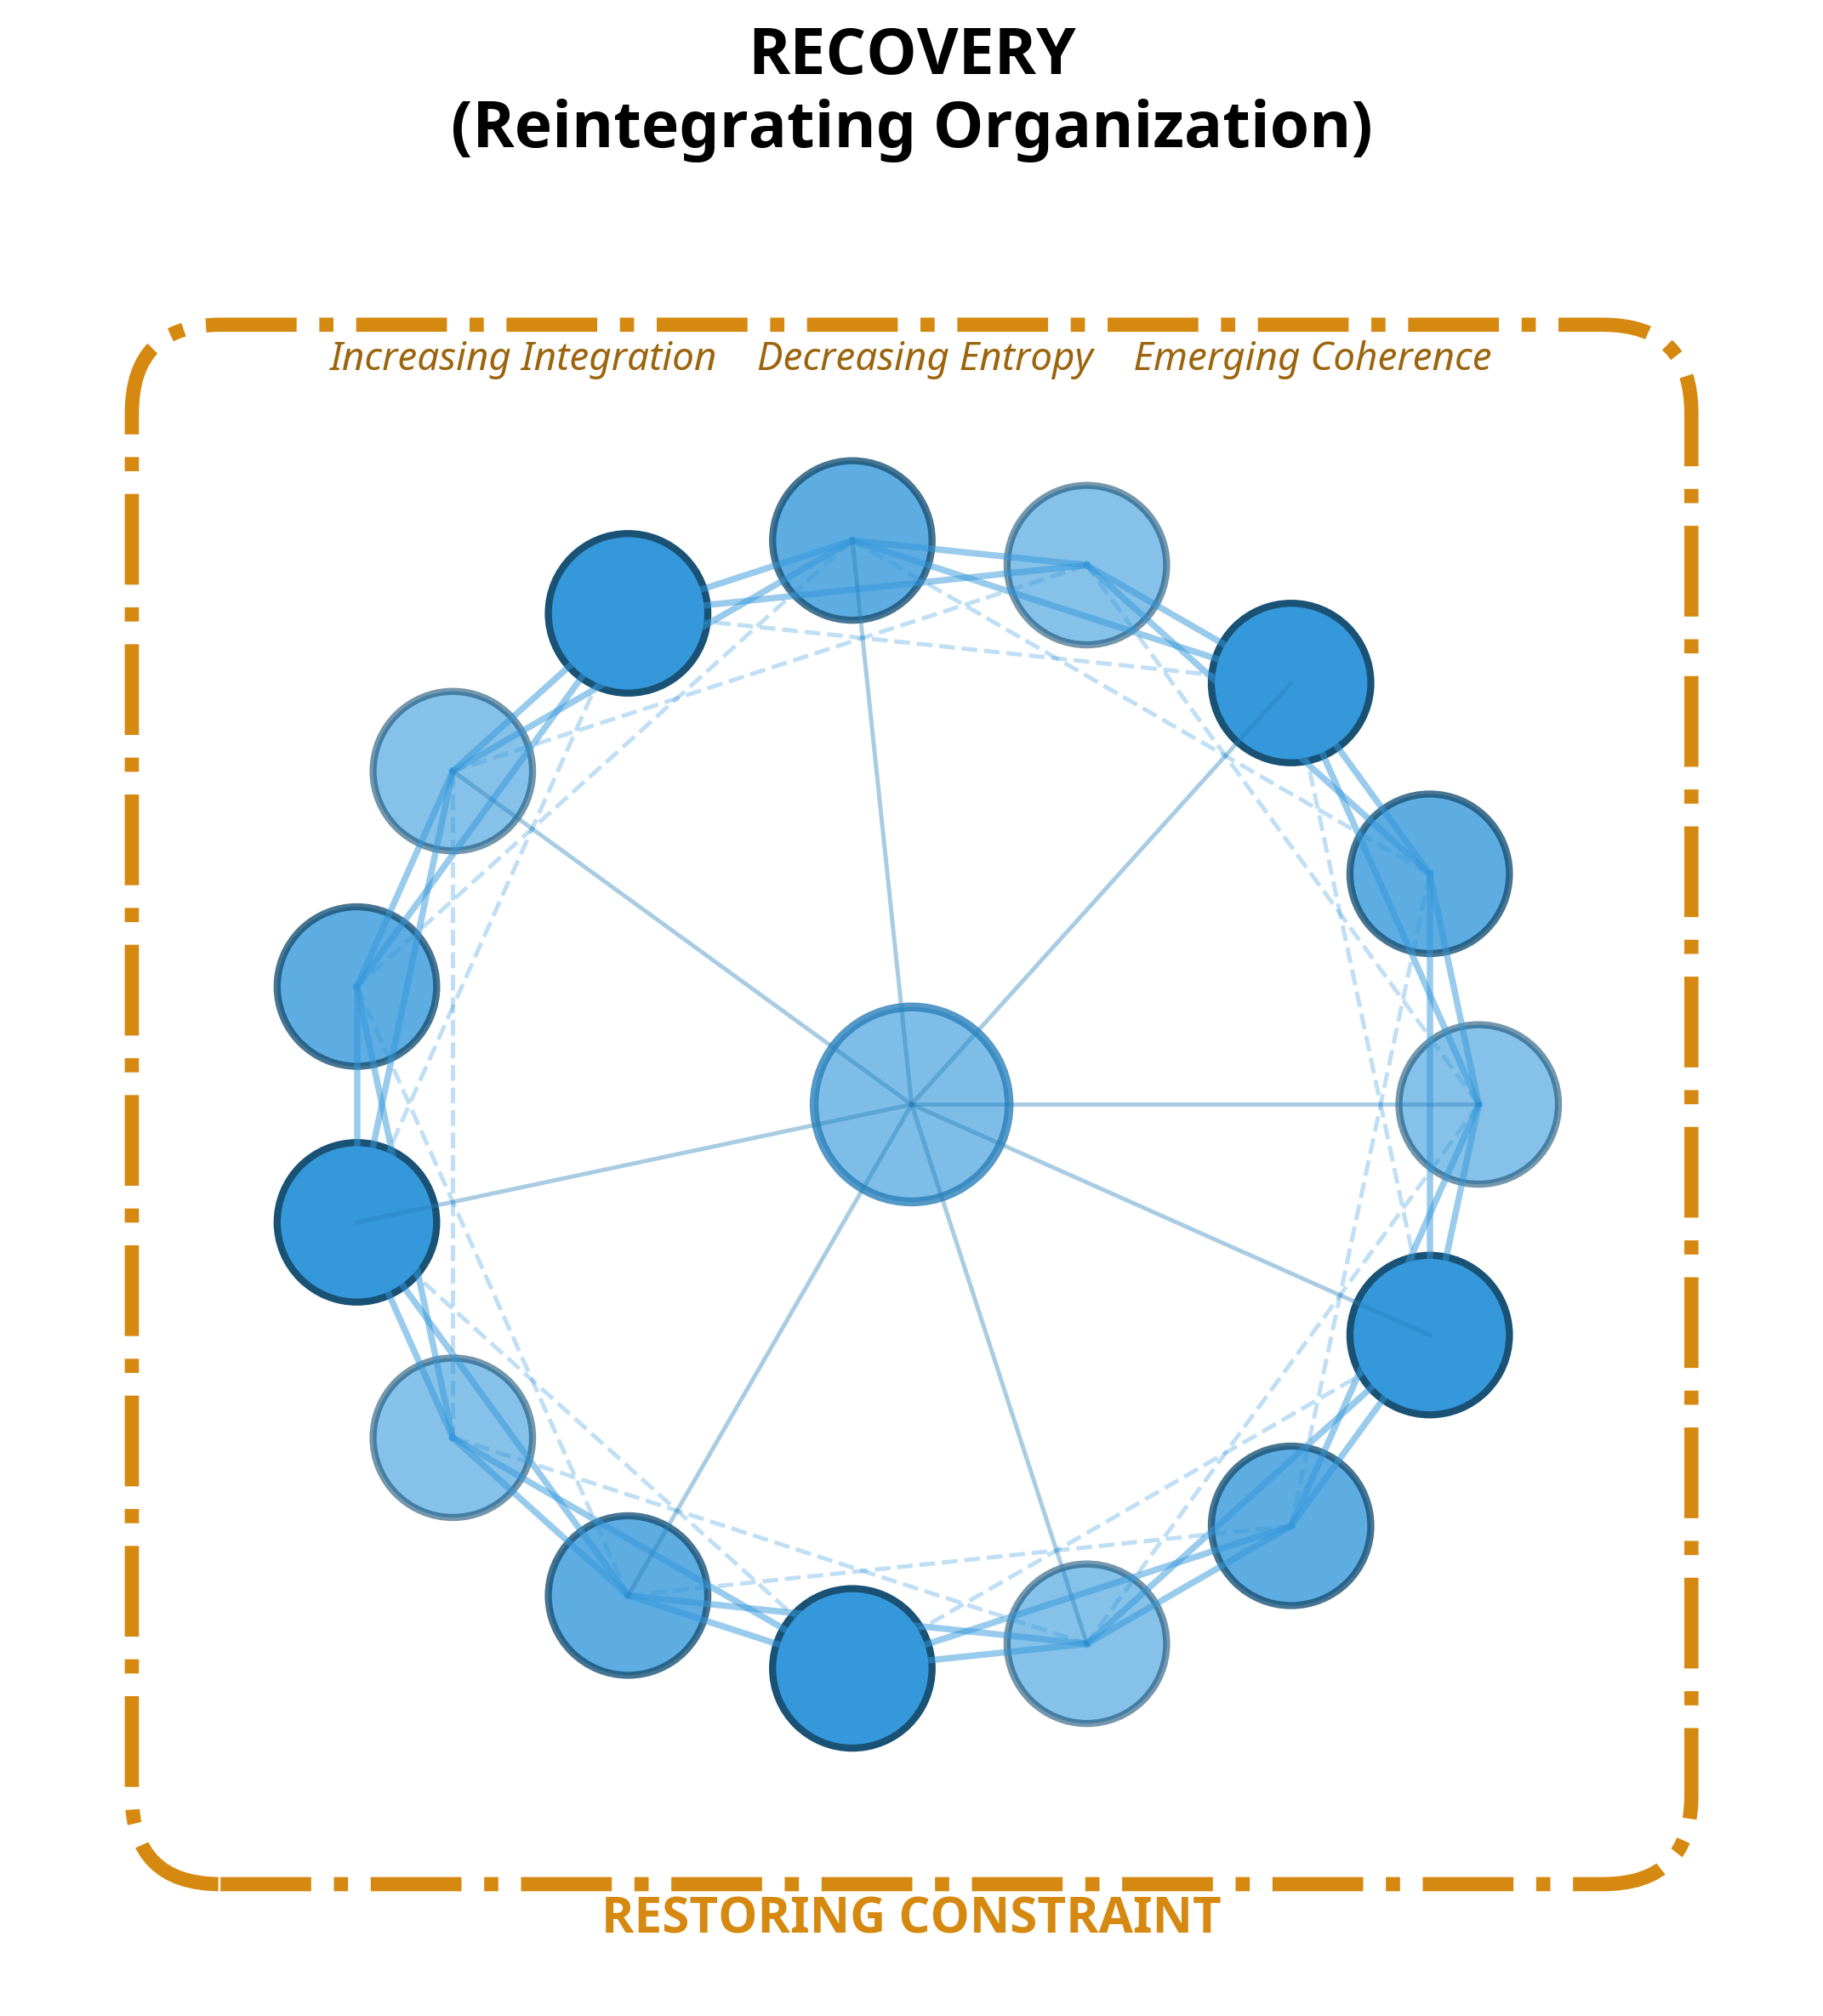
\includegraphics[width=0.7\textwidth]{figure3c_recovery.png}
\caption{Recovery and reintegration. Upon emergence from sleep or anesthesia, constraint systems gradually restore organizational coherence. Connections reform progressively as entropy decreases and integration increases. The dot-dash border represents restoring constraint conditions. Full conscious awareness reemerges when sufficient integration is reestablished. \textit{Author-created conceptual diagram; non-empirical; inspired by cited sources.}}
\label{fig:recovery}
\end{figure}

\section{Primitive Consciousness, Hallucination, and the Transition to Unified Awareness}

Historical and anthropological accounts suggest that unified conscious awareness may not have been a constant feature of human cognition. Julian Jaynes proposed that early human societies exhibited a form of mentality characterized by hallucinated commands and fragmented agency rather than by introspective self awareness \cite{jaynes1976}. While many details of this hypothesis remain debated, its central insight is relevant here: cognition can occur without stable integration or a unified sense of self.

From the perspective developed in this paper, such primitive or bicameral states can be understood as organizational regimes in which constraint is insufficient to enforce convergence. In these regimes, multiple internal models may coexist without integration, leading to experiences that are perceived as externally generated or authoritative. Hallucinations, in this context, are not treated as errors or malfunctions, but as natural consequences of systems operating with high entropy and weak pruning.

Neurobiological evidence supports the idea that hallucinations and fragmented cognition are associated with reduced integration and altered constraint. Psychotic states, certain seizure disorders, and dissociative conditions often involve disruptions in large scale connectivity and abnormal coordination across hemispheres and cortical regions \cite{friston2012, northoff2018}. These states mirror, at a neurophysiological level, the organizational features Jaynes described phenomenologically.

The transition from such fragmented cognition to unified conscious awareness therefore requires more than increased neural complexity or representational capacity. It requires mechanisms capable of reducing degrees of freedom, suppressing competing internal narratives, and stabilizing a dominant organizational regime. Within the framework developed here, this transition is driven by the maturation and alignment of external biological constraint systems that regulate entropy and enforce pruning.

Developmental evidence is consistent with this view. Early neural development is marked by exuberant connectivity and weak constraint, followed by progressive pruning and stabilization as metabolic, immune, and regulatory systems mature. Similarly, the gut brain biome undergoes substantial reorganization during early life, coinciding with critical periods of cognitive development and increasing behavioral coherence \cite{kundu2017, johnson2018}. These parallel trajectories suggest that the emergence of unified awareness reflects the coordinated action of neural and non neural systems rather than neural computation alone.

Importantly, this framework does not require that early humans or developing individuals lacked consciousness altogether. Rather, it suggests that conscious experience itself may have been less unified, less stable, and more prone to fragmentation in the absence of sufficient constraint. Unified awareness emerges when entropy gradients are appropriately bounded and cross system coupling stabilizes a single coherent field of experience.

In this light, Jaynes' historical account can be reinterpreted as a description of cognitive organization under weak constraint rather than as a claim about a fundamentally different mental substance. The transition to modern consciousness reflects not a sudden invention of awareness, but the gradual establishment of biological conditions capable of sustaining integrated, self consistent organization.

\subsection{Empirical Status of Microbial Oscillatory and Electromagnetic Activity}

This paper proposes that external biological constraint systems shape the space of viable neural configurations; the gut microbiome is included as one candidate constraint system. A critical question is whether microbial communities exhibit measurable oscillatory or electromagnetic activity that could plausibly couple, directly or indirectly, to neural organization. This subsection clarifies what is currently established in the literature; what is plausible but untested; and what remains unknown.

First, there is strong evidence that the microbiota--gut--brain axis influences neural development, immune tone, stress responsivity, and behavior through endocrine, immune, metabolic, and vagal pathways. These effects are widely supported; however, they do not by themselves imply that microbial electromagnetic frequencies act as direct modulators of neural pruning or conscious integration \cite{cryan2012, martin2018, cryan2019physrev}.\footnote{While electromagnetic and vibrational phenomena have been measured in biological materials and microbial systems under experimental conditions, no direct in vivo evidence currently demonstrates that gut microbiota generate a stable electromagnetic or oscillatory signal that modulates neural pruning, large-scale integration, or conscious awareness. The discussion of frequency in this paper is therefore framed as an experimentally motivated open question rather than an established mechanism.}

\begin{figure}[htbp]
\centering
\fbox{
  \parbox{0.8\textwidth}{
    \centering
    \vspace{2cm}
    Figure placeholder: Schematic of the gut-brain axis showing bidirectional communication pathways.
    \vspace{1cm}
    \\
    \textit{Source: Cryan et al. (2019), Martin et al. (2018)}
    \vspace{2cm}
  }
}
\caption{Placeholder for empirical figure illustrating the main communication routes between the gut microbiota and the brain. The figure would show the vagus nerve, enteric nervous system, immune system signaling, and metabolic pathways that constitute the gut-brain axis.}
\label{fig:placeholder_gutbrain}
\end{figure}

Second, there is literature showing that bacteria can respond to applied electromagnetic fields across a wide range of frequencies. Experimental work has examined changes in bacterial growth or antibiotic susceptibility under exposure to radiofrequency and microwave bands; more recent studies extend into higher frequencies, including tens of gigahertz. These findings demonstrate sensitivity and interaction with electromagnetic environments, but they do not establish that bacteria emit a stable intrinsic frequency signature that drives brain organization \cite{salmen2017hfemf, hegazy2025scirep}.

Third, terahertz and sub-terahertz methods are increasingly used to study vibrational properties of biological materials and to characterize cellular or membrane spectra. Work on low-terahertz vibrational behavior of biological membranes includes bacterial membrane models, indicating that biological structures can support organized dynamics in these bands. Separately, terahertz spectroscopy has been explored as a technique for detecting bacterial layers, spores, or cellular components. These domains support biophysical plausibility for higher-frequency organization in biological matter; they do not yet provide direct evidence of in vivo microbiome frequency signatures that modulate neural integration or pruning in humans \cite{luyet2023lowthzmembranes, datta2018spores}.

At present, the evidence base does not justify a claim that gut bacteria generate a specific oscillator frequency that can be identified as a pruning driver or as a consciousness modulator. The appropriate scientific position is that (i) microbial systems influence brain function via established biochemical and neural routes; (ii) bacterial systems can interact with electromagnetic fields across a wide range; and (iii) biological materials can exhibit organized behavior at higher-frequency bands that are measurable by terahertz methods. The open question is whether any of these measurable microbial or biophysical frequency phenomena couple meaningfully to the neural signatures associated with integration, sleep-state transitions, pruning trajectories, or stability of self-modeling.

\textbf{Literature Search Methodology and Results.} A systematic search was conducted across PubMed, Google Scholar, Nature, Science Direct, and IEEE using the following terms: bacterial electromagnetic emission, microbial oscillatory activity, THz terahertz spectroscopy bacteria, bacterial membrane vibration, microbiome electromagnetic signaling, and gut bacteria frequency neural. The search yielded the following categories of evidence:

\textit{Category 1: Bacterial response to external electromagnetic fields.} Multiple studies document that bacteria respond to externally applied electromagnetic fields across frequencies from megahertz to gigahertz ranges \cite{hegazy2025scirep}. These demonstrate sensitivity to electromagnetic environments but do not demonstrate endogenous emission.

\textit{Category 2: THz spectroscopy of bacteria.} Studies use external terahertz radiation to probe bacterial structure and detect microorganisms \cite{luyet2023lowthzmembranes}. These are detection technologies, not measurements of endogenous bacterial emission.

\textit{Category 3: Theoretical proposals.} Historical proposals by Fr\"ohlich and others predict coherent oscillations in biological membranes in the gigahertz to terahertz range \cite{froehlich1968}. These remain theoretical predictions without direct experimental confirmation in gut microbiota.

\textit{Category 4: Microbiome-microglia-pruning pathway.} In contrast to the electromagnetic hypothesis, substantial evidence exists for gut microbiota influencing synaptic pruning through microglia via immune signaling, complement system mediation, and metabolic pathways \cite{eltokhi2020, hao2024, abdelhaq2019}. This pathway is well documented and does not require electromagnetic signaling.

\textbf{Critical Finding: Evidence Gap.} The search reveals that while bacteria respond to electromagnetic fields and THz spectroscopy can characterize bacterial structures, no direct experimental evidence currently demonstrates that gut microbiota emit electromagnetic signals that influence neural organization or development. The microbiome-brain connection operates through established biochemical, immune, and neural routes rather than through demonstrated electromagnetic coupling.

This motivates a concrete research direction: paired longitudinal measurements combining microbiome profiling with neural measures of integration and state transitions. If a microbial frequency-linked signal exists and is functionally relevant, it should correlate with reproducible changes in established neural markers of integration and complexity, and it should vary systematically with known modulators such as sleep architecture, anesthesia transitions, inflammation, and developmental pruning windows. Until such evidence exists, frequency coupling should be treated as a plausible but unverified mechanism and framed as an experimental target rather than a conclusion.

\section{Frequency, Modulation, and Cross Scale Biological Coupling}

Biological organization unfolds across a wide range of temporal and energetic scales. Neural dynamics typically emphasized in consciousness research operate in low frequency regimes accessible to electroencephalography and related methods. These rhythms are clearly relevant to cognition and awareness, yet they represent only a narrow band of biological activity. Molecular, cellular, and metabolic processes operate on much faster timescales and involve forms of organization that are not directly observable through conventional neural recording techniques.

At the molecular level, biological systems exhibit structured vibrational and electromagnetic activity associated with protein conformational dynamics, membrane oscillations, ion transport, and collective behavior in aqueous environments. These processes naturally extend into the gigahertz and terahertz frequency ranges and have been proposed as contributors to long range coherence and biological order \cite{froehlich1968, pokorny2004}. While such activity is not typically treated as part of neural computation, it may nevertheless influence the energetic and organizational landscape in which neural dynamics unfold.

Bacterial systems provide a particularly relevant example. Microbial communities exhibit coordinated metabolic activity, collective oscillations, and electromagnetic signaling linked to ion flux and energy transfer. These processes are shaped by temperature, pressure, chemical gradients, and environmental conditions, suggesting that frequency dependent organization is tightly coupled to thermodynamic regulation. Although direct evidence linking bacterial frequency activity to neural coherence remains limited, the existence of structured high frequency biological organization motivates its consideration as a potential modulatory substrate rather than as a cognitive mechanism.

Within the framework developed here, frequency organization is not treated as a generator of consciousness, nor is a specific consciousness frequency proposed. Instead, frequency dependent biological processes are considered as contributors to constraint and stabilization. High frequency organization may shape the boundary conditions under which lower frequency neural integration occurs, much as slow metabolic processes constrain faster neural signaling. In this view, cross scale coupling allows biological systems to maintain coherence without requiring direct synchronization across all levels.

This perspective aligns with observations from neuromodulation and anesthesia studies. Perturbations applied at relatively coarse spatial and temporal scales can collapse conscious awareness by disrupting integration, even though fine grained neural and molecular activity continues. Conversely, restoration of consciousness requires not only resumption of neural firing, but the reestablishment of appropriate coupling across scales. Frequency organization may therefore function as an enabling background that supports or destabilizes integration depending on its alignment with other constraints.

The possibility of cross scale frequency coupling also resonates with proposals that consciousness exhibits compressed representational properties. Conscious experience reflects a stabilized representation of underlying biological dynamics rather than a direct readout of all activity. This compression depends on selective coupling and decoupling across scales, allowing the system to suppress irrelevant degrees of freedom while preserving coherence. The field metaphor captures how biological systems construct stable experiential states from complex underlying processes.

Finally, this framework remains compatible with sub neural proposals such as those involving microtubules and related structures, which posit that non classical or sub cellular processes may contribute to conscious organization \cite{penrose2014}. Rather than competing with neural level theories, such proposals can be understood as identifying additional layers of constraint or coupling that influence integration. Whether these layers are necessary, sufficient, or merely modulatory remains an open empirical question. The present framework emphasizes that any such contributions must operate by shaping entropy gradients and stabilizing organization rather than by introducing isolated causal mechanisms.

In summary, frequency dependent biological organization provides a plausible avenue for understanding how constraint and coherence are maintained across scales. While much remains to be empirically established, treating frequency as a modulatory and stabilizing factor rather than as a direct cause of consciousness allows for cautious exploration without overstatement. This approach integrates neural, molecular, and ecological processes into a unified biological picture of conscious organization.

\begin{figure}[htbp]
\centering
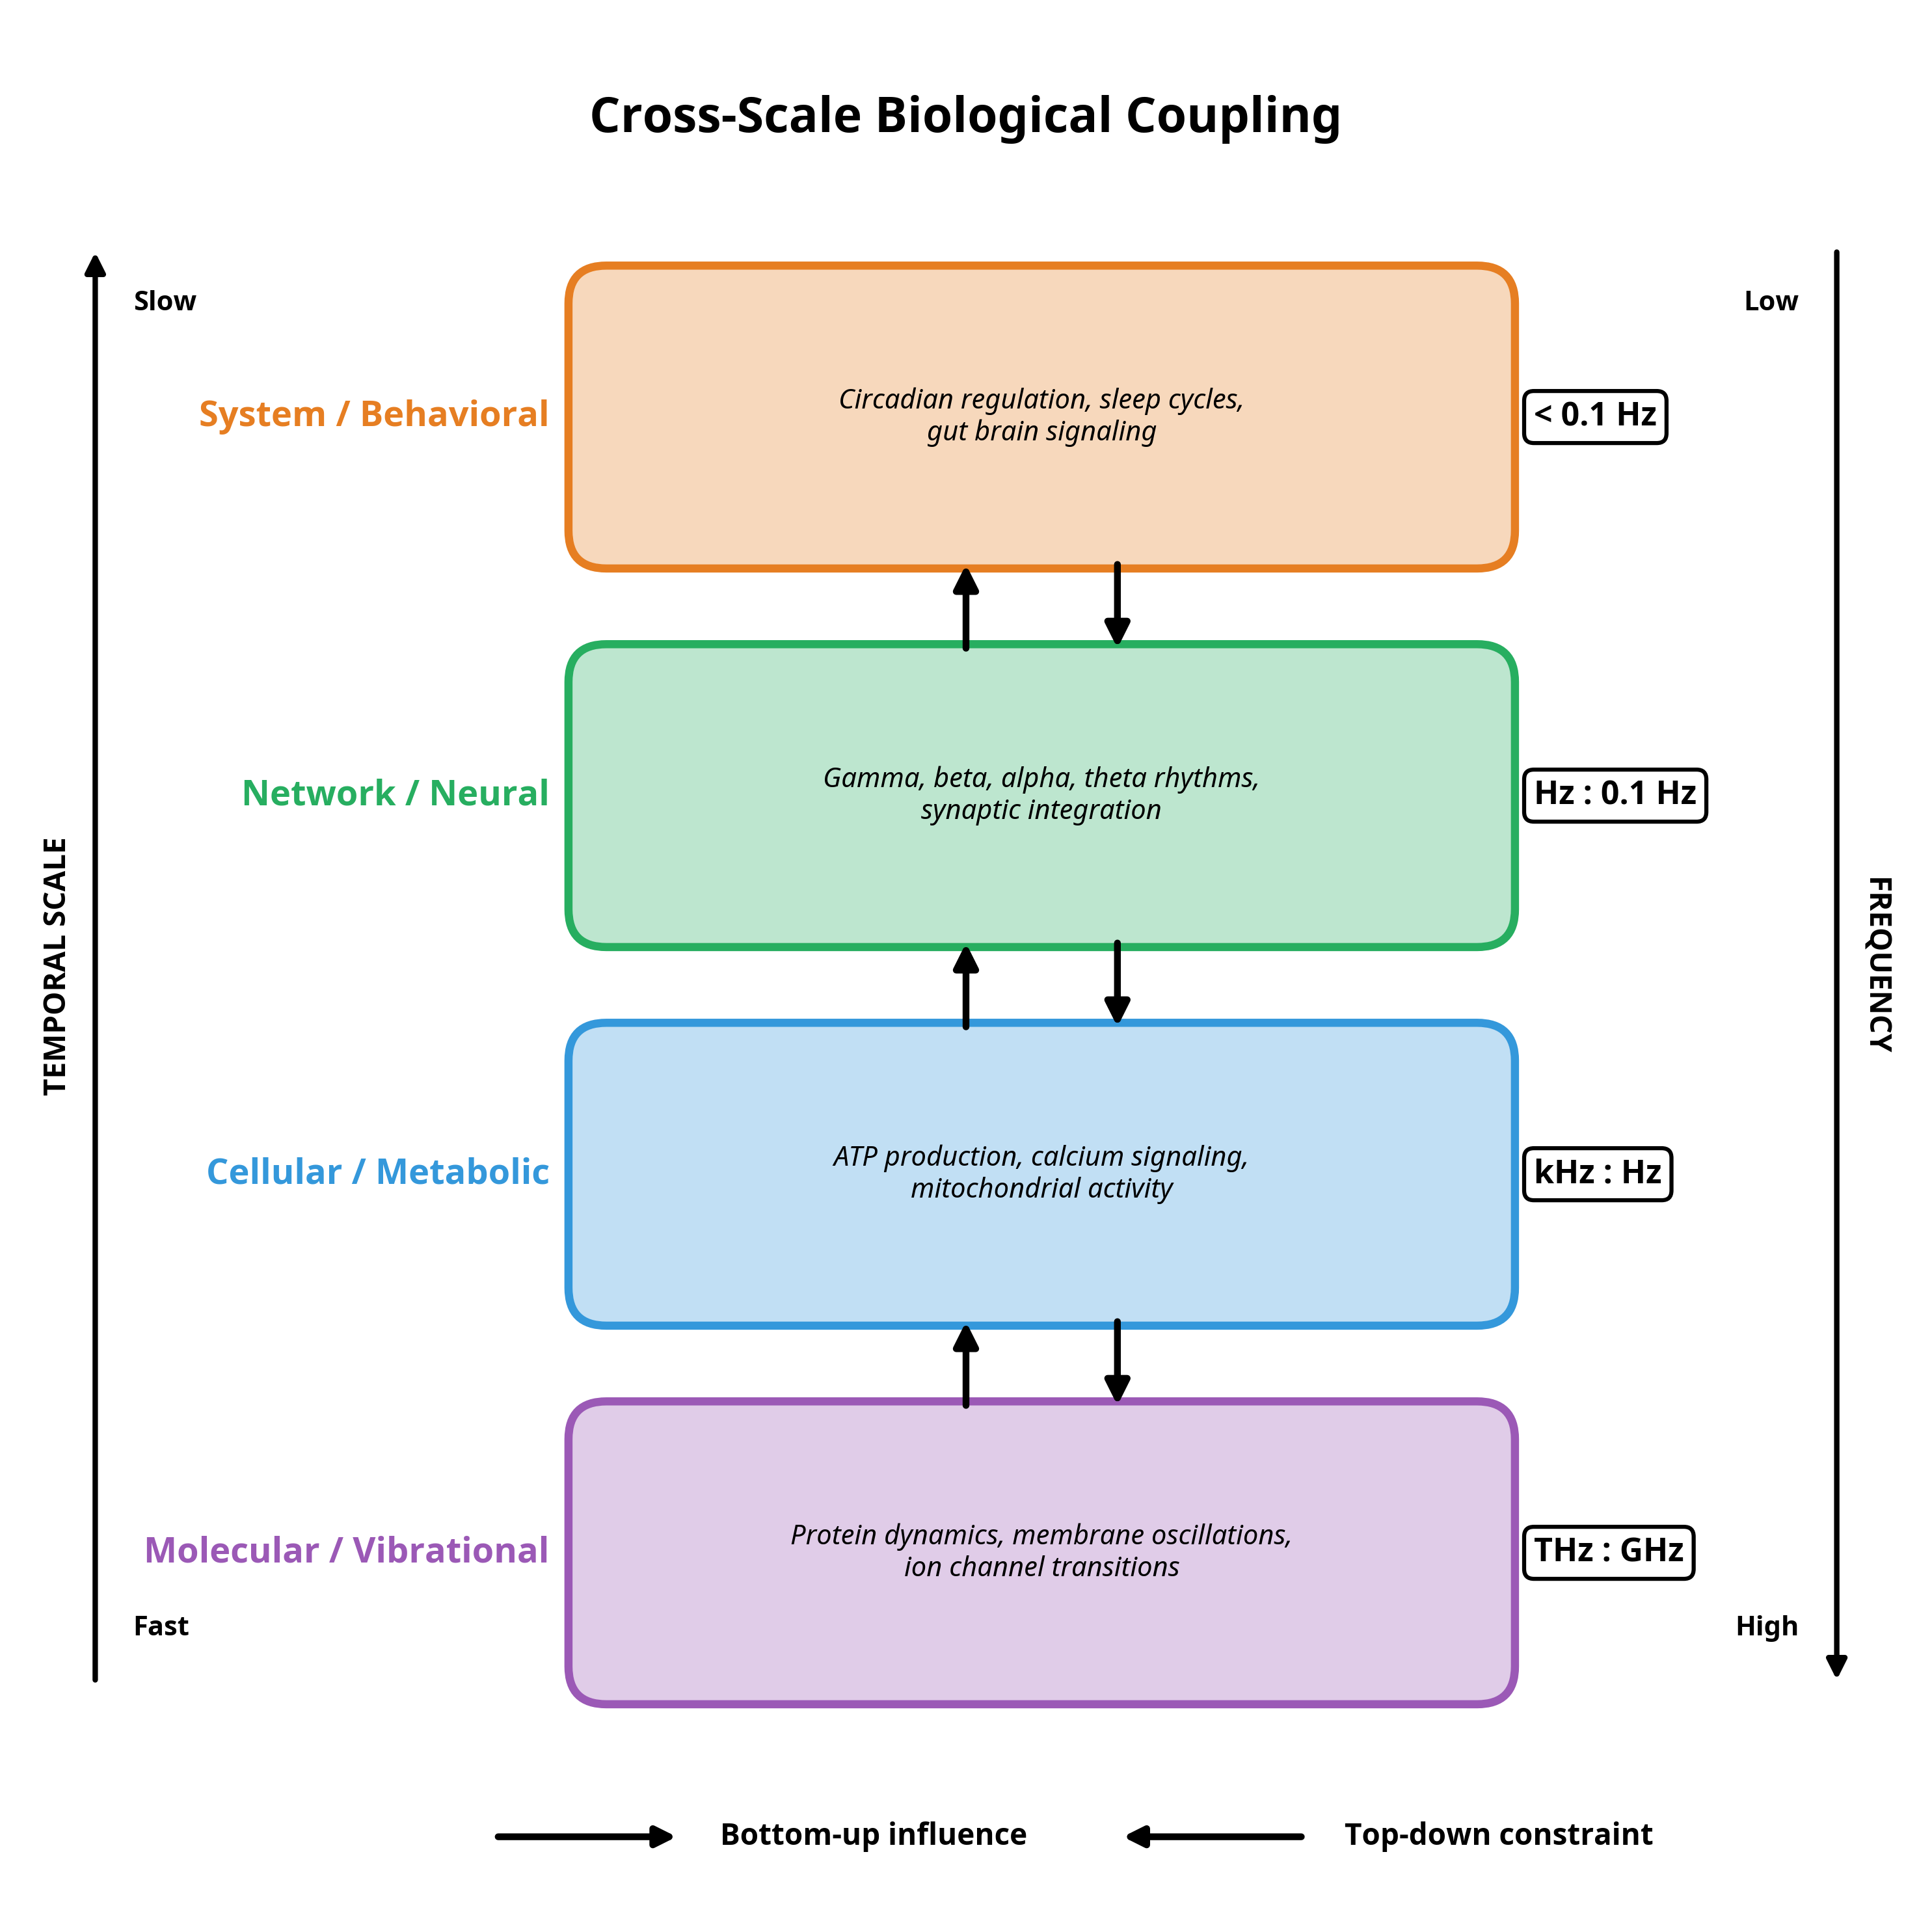
\includegraphics[width=0.85\textwidth]{figure4_crossscale.png}
\caption{Cross-scale biological coupling. Biological organization spans multiple temporal and frequency scales, from fast molecular and vibrational processes (terahertz to gigahertz) through cellular and metabolic activity (kilohertz to hertz) to neural network dynamics (hertz to sub-hertz) and slow system-level behavioral regulation (below 0.1 hertz). Bidirectional arrows indicate bottom-up influence and top-down constraint between adjacent scales. This hierarchical coupling allows constraint to propagate across levels, enabling high-frequency molecular processes to modulate the boundary conditions for lower-frequency neural integration, while slow regulatory processes shape the overall organizational landscape. \textit{Author-created conceptual diagram; non-empirical; inspired by cited sources.}}
\label{fig:crossscale}
\end{figure}

\section{Predictions and Experimental Directions}

The framework developed in this paper makes several testable predictions concerning the biological conditions required for conscious organization. These predictions do not depend on identifying a single neural locus or frequency, but instead focus on organizational properties, constraint mechanisms, and cross scale coupling. Importantly, many of these predictions are accessible using existing experimental tools.

First, if conscious awareness depends on entropy regulation and global constraint, then manipulations that weaken or strengthen embodied constraint systems should systematically alter measures of integration. Network level metrics such as effective connectivity, perturbational complexity, and long range coherence should vary not only with neural activity, but with metabolic, immune, and regulatory state. This prediction aligns with observations that systemic inflammation, metabolic disruption, and circadian misalignment can alter conscious experience even in the absence of focal neural damage \cite{koch2019, northoff2018}.

Second, interventions targeting the gut brain biome should influence neural integration in ways that are not reducible to localized neurotransmitter effects. Changes in microbiome composition are predicted to modulate large scale network organization, pruning dynamics, and the stability of integrated states over time. Longitudinal studies combining microbiome analysis with neuroimaging and electrophysiology could test whether shifts in microbial ecology correlate with changes in integration metrics, sleep architecture, or susceptibility to fragmentation and hallucination \cite{cryan2012, foster2013}.

Third, sleep and anesthesia provide controlled contexts for testing constraint based predictions. The framework predicts that loss and restoration of consciousness should correlate with changes in entropy gradients and cross scale coupling rather than with absolute levels of neural firing. Measures of synaptic downscaling, metabolic clearance, and slow regulatory processes during sleep should predict subsequent restoration of integration more reliably than local activity measures alone \cite{tononi2014, casali2013}.

Fourth, frequency dependent biological organization can be explored cautiously through indirect measures. Rather than attempting to directly detect high frequency neural oscillations, studies can examine whether perturbations at molecular or metabolic levels influence lower frequency neural integration. For example, temperature modulation, pressure changes, or metabolic interventions may alter network stability in ways consistent with changes in constraint rather than direct neural excitation. Such experiments would help clarify whether high frequency biological processes act as modulatory backgrounds rather than as discrete oscillators.

Fifth, neuromodulation techniques such as transcranial magnetic stimulation offer a means of probing the limits of admissible organization. By systematically varying stimulation parameters and measuring the resulting changes in integration and complexity, it may be possible to map the boundary between conscious and non conscious organizational regimes. These boundaries are predicted to depend on the system's overall regulatory state rather than on stimulation alone \cite{massimini2005, casali2013}.

Finally, computational and modeling approaches can be used to explore the implications of constraint driven organization. Models that incorporate entropy regulation, pruning, and multi scale coupling are predicted to exhibit phase transitions between fragmented and unified regimes. While such models do not imply that the brain is literally a simulation, they can capture properties of compression, stability, and selective representation that characterize conscious experience.

Together, these predictions emphasize that consciousness is best studied as an emergent property of constrained biological organization. Progress will require integrating neural, metabolic, immune, and ecological data rather than focusing exclusively on isolated neural mechanisms. By grounding theoretical claims in experimentally accessible domains, this framework aims to bridge abstract theories of consciousness with concrete biological processes.

\section{Biological Organization, Entropy Gradients, and Frequency-Based Neural Pruning}

Julian Jaynes' bicameral mind hypothesis provides a historically grounded account of early human consciousness characterized by hallucinations, externally attributed cognition, and the absence of stable self-reflection. While Jaynes convincingly documents this transition through linguistic and anthropological evidence, his framework does not identify the biological mechanism that enabled the emergence of unified subjective experience. This section argues that the missing mechanism is large-scale biological organization driven by neural pruning, entropy gradients across brain hierarchies, and frequency-based regulation, including contributions from gut microbiota and endogenous physiological signaling.

\subsection{From Bicameral Cognition to Organized Self-Reflection}

The transition from hallucination-dominated cognition to structured self-reflection required a reorganization of neural architecture rather than a sudden cultural or symbolic shift. Prior to sufficient organization, cognitive activity lacked a stable integration point, resulting in fragmented or externally interpreted experiences. Neural pruning reduced degrees of freedom in higher cortical regions, allowing information to be consolidated and recursively referenced.

This organizational shift postdated the bicameral phenomena described by Jaynes and created the structural conditions necessary for internally generated self-models. Conscious self-reflection emerged not simply because language changed, but because biological organization reached a threshold where information could be compressed, stabilized, and integrated.

The historical transition described by Jaynes can thus be reinterpreted as a period in which internal cognitive attractors existed without sufficient external biological constraint to stabilize a dominant self-referential configuration. The emergence of organized pruning and constraint alignment enabled the collapse from competing attractors into a single integrated experiential regime. This reframing connects the anthropological evidence to the biological mechanisms developed throughout this paper, suggesting that the bicameral to unified consciousness transition reflects an organizational phase change rather than a purely cultural or linguistic evolution.

\subsection{Gut Microbiota, Endogenous Frequencies, and Neural Organization}

Research on the gut-brain axis demonstrates that gut microbiota actively influence neural development, plasticity, and long-term regulation. Microbial populations modulate neurotransmitter availability, immune signaling, vagal nerve activity, and oscillatory brain dynamics. These processes contribute to the slow shaping and stabilization of neural networks over developmental and evolutionary timescales.

Several studies show that specific microbial profiles are associated with improved motor and cognitive outcomes in Parkinson's disease and other disorders involving disrupted neural coordination \cite{sampson2016}. This supports the hypothesis that microbial signaling participates in regulating neural organization and pruning, indirectly shaping the entropy structure of the brain.

Rather than acting as a direct cause of consciousness, gut bacteria function as distributed biological regulators that influence how neural systems organize, stabilize, and filter information.

\subsection{Pruning Failure, Schizophrenia, and Misaligned Organization}

Pathological cases further support the role of organization and pruning in conscious experience. Schizophrenia is increasingly understood as a disorder involving disrupted or mistimed synaptic pruning, resulting in misaligned integration across cortical hierarchies \cite{sekar2016}. Hallucinations and fragmented cognition reappear when filtering mechanisms fail, resembling features of bicameral cognition but arising from structural dysfunction rather than historical development.

This suggests that organized pruning is not merely developmental optimization, but a prerequisite for stable subjective experience.

\subsection{Entropy Gradients Across Brain Hierarchies}

Neural organization follows a hierarchical structure in which different brain regions exhibit different degrees of freedom and informational density. Lower brain regions, including the brainstem and cerebellum, support high degrees of freedom and interface directly with bodily regulation and environmental interaction. Damage to these regions leads to loss of autonomy or death.

Intermediate regions, such as the temporal and limbic systems, perform filtering, sensory integration, and emotional weighting. Higher cortical regions, particularly the prefrontal cortex, compress and stabilize information into a unified experiential perspective.

This hierarchical organization explains why frontal damage often redistributes cognitive function, while disruption of lower structures results in catastrophic failure.

\subsection{Surgical and Rewiring Evidence for Filtering}

Clinical and experimental cases strongly support a filtering-based model of consciousness. Amygdala lesions alter emotional processing without eliminating awareness. Corpus callosotomy separates hemispheric integration while preserving local conscious experience. Optic chiasm severing and sensory remapping experiments demonstrate that perception reorganizes according to structural constraints rather than fixed representations.

These findings indicate that consciousness depends on how information is filtered and integrated, not on any single anatomical location.

\subsection{The Brain as an Interface Rather Than a Generator}

The brain functions as an interface that filters, organizes, and stabilizes information rather than generating consciousness outright. This view aligns with theories of recursive self-reference, emergent pattern formation, and computational irreducibility. Conscious experience arises from organized constraint, not from raw processing power.

\subsection{Frequency Regulation and Deep Organizational Mechanisms}

Most existing treatments target chemical signaling or low-frequency electrical activity. However, experimental evidence suggests that higher-frequency electromagnetic interactions, including terahertz-scale effects, influence protein dynamics, ion channel behavior, and neural coherence. These mechanisms may regulate deeper layers of biological organization that current interventions do not address.

This provides a plausible framework for understanding how frequency-based regulation contributes to long-term neural organization and pruning.

\subsection{Limits of Anesthesia-Based Models of Consciousness}

Anesthesia suppresses neural output but does not explain subjective experience, solipsism, or individual variability. Qualia arise because no two brains share identical microstructure. Genetic, molecular, and developmental variations alter how information is filtered and integrated, producing distinct experiential outcomes.

Although humans share broadly similar networks, infinitesimal differences in organization generate meaningful differences in perception and experience. Consciousness studies must therefore extend beyond anesthesia models to address structural and organizational mechanisms.

\section{Limitations}

It is important to state the limitations of this framework directly. First, the role of the gut-brain axis is presented as a plausible source of constraint, but the evidence remains largely correlational. While the microbiome influences neural development and function, the specific mechanisms by which it might regulate global integration are not yet established. Second, the application of Gödel's theorems to biological systems is a high-level interpretation, not a direct mathematical proof. It serves to motivate the need for external constraint, but does not by itself specify the nature of that constraint. Third, the discussion of high-frequency biological phenomena is exploratory. While biophysically plausible, there is currently no direct evidence that microbial oscillatory activity acts as a functional constraint on neural dynamics in vivo. The framework is therefore best understood as a conceptual model designed to guide experimental investigation, not as a complete or final theory.

\section{Discussion and Conclusion}

This paper has advanced a conservative biological framework to address the question of how biological systems achieve stable, unified awareness. We have argued that consciousness is best understood as a stabilized organizational regime and that neural systems require external biological constraints to regulate entropy and enforce large-scale integration. This framework was supported by a review of evidence from sleep and anesthesia, perturbational complexity studies, and developmental neuroscience. We also examined the formal limits of self-referential systems to motivate the need for external constraint. Our literature search demonstrated that while the gut-brain axis influences neural function through established biochemical pathways, there is currently no direct evidence for a microbial electromagnetic or oscillatory signal that drives neural organization. This work therefore distinguishes between what is empirically supported and what remains a targeted experimental opportunity. By grounding the study of consciousness in experimentally accessible mechanisms of constraint and integration, this framework moves beyond a search for localized neural correlates and toward an investigation of the distributed, multi-scale processes that support biological integrity.

\appendix
\section{Appendix: Methodological Considerations}

This appendix addresses methodological considerations relevant to the framework developed in this paper. The arguments presented do not depend on any single empirical finding or experimental technique, but rather on the convergence of evidence from multiple domains. This convergence strengthens the case for constraint based approaches to consciousness while acknowledging the limitations of current methods.

Measures of integration such as the perturbational complexity index provide a useful but incomplete picture of conscious organization. These measures capture certain aspects of network dynamics but may not fully reflect the contribution of non neural constraint systems. Future methodological development should aim to incorporate metabolic, immune, and ecological variables alongside neural measures.

The study of gut brain interactions presents particular methodological challenges. Microbiome composition is highly variable across individuals and sensitive to diet, environment, and other factors. Longitudinal designs with careful control of confounding variables will be essential for establishing causal relationships between microbial ecology and neural integration.

Finally, the exploration of high frequency biological organization requires instrumentation and analytical approaches that are not yet standard in neuroscience. Terahertz spectroscopy and related techniques have been applied in biophysics but have not been systematically integrated with consciousness research. Interdisciplinary collaboration will be necessary to develop appropriate methods for investigating cross scale coupling in living systems.

\section{Limitations}

It is important to acknowledge the limitations of this framework. First, the proposed role of the gut-brain axis as a constraint layer is based on established bidirectional signaling pathways, but its specific contribution to the global regulation of neural integration remains correlational. Direct causal evidence linking microbial state to changes in cortical complexity is currently lacking. Second, while the formal argument for external constraint is logically grounded, its application to biological systems is a high-level interpretation; the precise mapping between formal systems and neural dynamics is an area of active research. Finally, the empirical evidence for microbial oscillatory or electromagnetic activity is still in its infancy. The studies cited here demonstrate that such effects are plausible and measurable, but they do not provide evidence of a functional role in neural regulation. The framework presented here should therefore be seen as a theoretical and experimental guide, not a definitive model.


\bibliography{references}
\bibliographystyle{unsrtnat}

\end{document}
